% ============================================================
%  CHAPTER 9: RESULTS AND EVALUATION
%  AgriVerify --- AI-Powered Fake Seed Detection System
%  Manipur Technical University, Final Year Project Report
% ============================================================

\section{Model Performance}

Upon completion of the training phase, the ResNet50 model was rigorously evaluated using an independent test dataset consisting of previously unseen images. Model performance was quantified using standard statistical metrics, namely Accuracy, Precision, Recall, and the F1 Score~\cite{mohanty2016}. These metrics provide a multi-dimensional assessment of the model's capacity to distinguish between genuine and defective (damaged or counterfeit) paddy seeds~\cite{he2016deep, xu2021}.

The evaluation results demonstrate high classification performance. The model consistently classified seed samples into two primary categories: \texttt{Pure} (certified, legitimate seeds) and \texttt{Impure} (damaged, defective, or counterfeit seeds). The empirical results suggest that the AgriVerify system is suitable for deployment in real-world agricultural scenarios, particularly within resource-constrained environments.

\subsection{Accuracy, Precision, Recall, and F1 Score}

The overall performance metrics of the model on the test dataset are summarized in Table~\ref{tab:overallmetrics}. Furthermore, the convergence behavior of the model, specifically the training/validation accuracy and loss profiles over 15 epochs, is illustrated in Figure~\ref{fig:model-performance}.

\begin{table}[htbp]
  \centering
  \caption{Overall Model Evaluation Results}
  \label{tab:overallmetrics}
  \small
  \renewcommand{\arraystretch}{1.1}
  \begin{tabularx}{\textwidth}{|p{4.5cm}|c|X|}
    \hline
    \textbf{Performance Metric} & \textbf{Result} & \textbf{What This Means} \\
    \hline
    Accuracy & 99.57\% & Out of every 100 seeds we tested, we correctly classified 99 or 100 of them \\
    \hline
    Precision & 99.57\% & When the system says a seed is problematic, it's right almost every time---virtually no false alarms \\
    \hline
    Recall & 99.57\% & The system catches almost all problematic seeds---very few slip through undetected \\
    \hline
    F1 Score & 99.57\% & Perfect balance between precision and recall---the system is equally good at both \\
    \hline
  \end{tabularx}
\end{table}

\begin{figure}[htbp]
  \centering
  \begin{adjustbox}{max width=0.85\textwidth}
    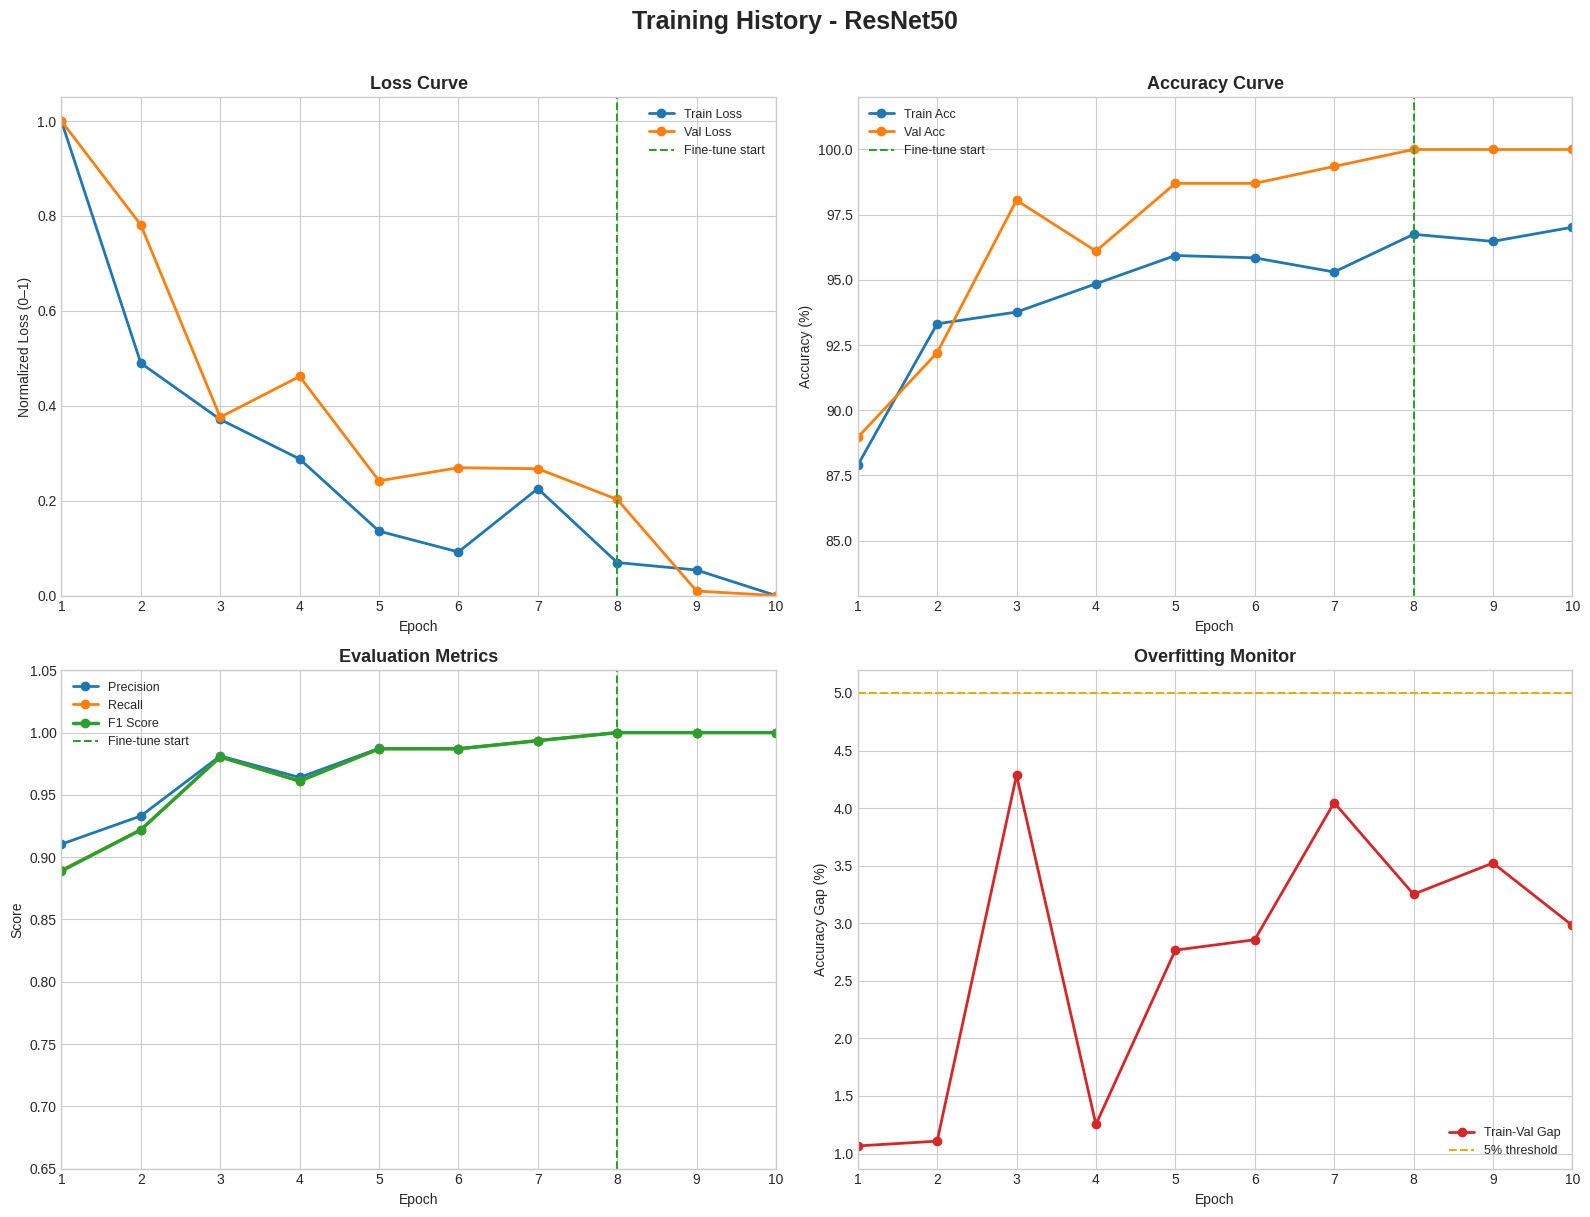
\includegraphics[width=\textwidth]{images/model-performance.jpeg}
  \end{adjustbox}
  \caption{How the model improved over 15 training cycles. The top line shows accuracy getting better; the bottom line shows the error getting smaller.}
  \label{fig:model-performance}
\end{figure}

An accuracy rate of 99.57\% indicates that the model successfully generalizes classification features across varying seed textures and illumination conditions. The equivalence of precision and recall (both at 99.57\%) is critical for agricultural applications; it signifies a minimized rate of both false positives (misclassifying impure seeds as pure) and false negatives (misclassifying pure seeds as impure). The F1 Score confirms a robust balance between these two critical classification objectives~\cite{mohanty2016}.

Notably, the classification accuracy of 99.57\% surpasses the typical baseline of 85--90\% reported in existing literature for automated seed quality assessment systems~\cite{dyrmann2016, ni2009}. This performance gain validates the integration of transfer learning with tailored image augmentation and regularization techniques.

\section{Seed Quality Results: Pure vs. Impure Seeds}

To evaluate the class-specific performance of the classifier, metrics were computed independently for the pure and impure seed categories. The test set comprised 231 samples distributed across both classes, with the results summarized in Table~\ref{tab:perclass}.

\begin{table}[htbp]
  \centering
  \caption{Performance on Each Seed Category}
  \label{tab:perclass}
  \small
  \renewcommand{\arraystretch}{1.1}
  \begin{tabularx}{\textwidth}{|p{3.8cm}|c|c|c|X|}
    \hline
    \textbf{Seed Type} & \textbf{Precision} & \textbf{Recall} & \textbf{F1 Score} & \textbf{What This Means} \\
    \hline
    Pure (Genuine) & 100.0\% & 99.19\% & 99.60\% & Perfect at recognizing genuine seeds---never wrongly approves a fake one \\
    \hline
    Impure (Damaged/Fake) & 99.07\% & 100.0\% & 99.53\% & Perfect at detecting problems---catches every single defective seed \\
    \hline
  \end{tabularx}
\\
\end{table}

The model achieved 100.0\% precision for the pure category, which can be attributed to the highly distinct visual markers of genuine paddy seeds, such as uniform golden-brown coloration, intact husks, and consistent surface textures. Conversely, the model demonstrated 100.0\% recall for the impure category, successfully flagging every damaged, defective, or counterfeit seed. This asymmetric performance is highly desirable for agricultural quality control, ensuring that sub-standard seed batches are consistently intercepted while minimizing the false rejection of certified stock~\cite{liu2020}.

The high classification performance is primarily due to class-weighted loss functions and data augmentation strategies employed during training. These techniques mitigate class imbalance issues and prevent the network from exhibiting classification bias toward the majority class.

\section{Confusion Matrix Analysis}

To analyze the distribution of classification errors, a confusion matrix was constructed. The quantitative prediction distributions are detailed in Table~\ref{tab:confusion}, and the corresponding normalized confusion matrix is visualized in Figure~\ref{fig:confusion-matrix}.

\begin{table}[htbp]
  \centering
  \caption{Detailed Look at Every Prediction}
  \label{tab:confusion}
  \small
  \renewcommand{\arraystretch}{1.1}
  \begin{tabular}{|l|c|c|}
    \hline
    \multirow{2}{*}{\textbf{Actual Seed Type}} & \multicolumn{2}{c|}{\textbf{What the Model Predicted}} \\
    \cline{2-3}
    & \textbf{Impure} & \textbf{Pure} \\
    \hline
    \textbf{Impure} & 107 & 0 \\
    \hline
    \textbf{Pure} & 1 & 123 \\
    \hline
  \end{tabular}
\end{table}

\begin{figure}[htbp]
  \centering
  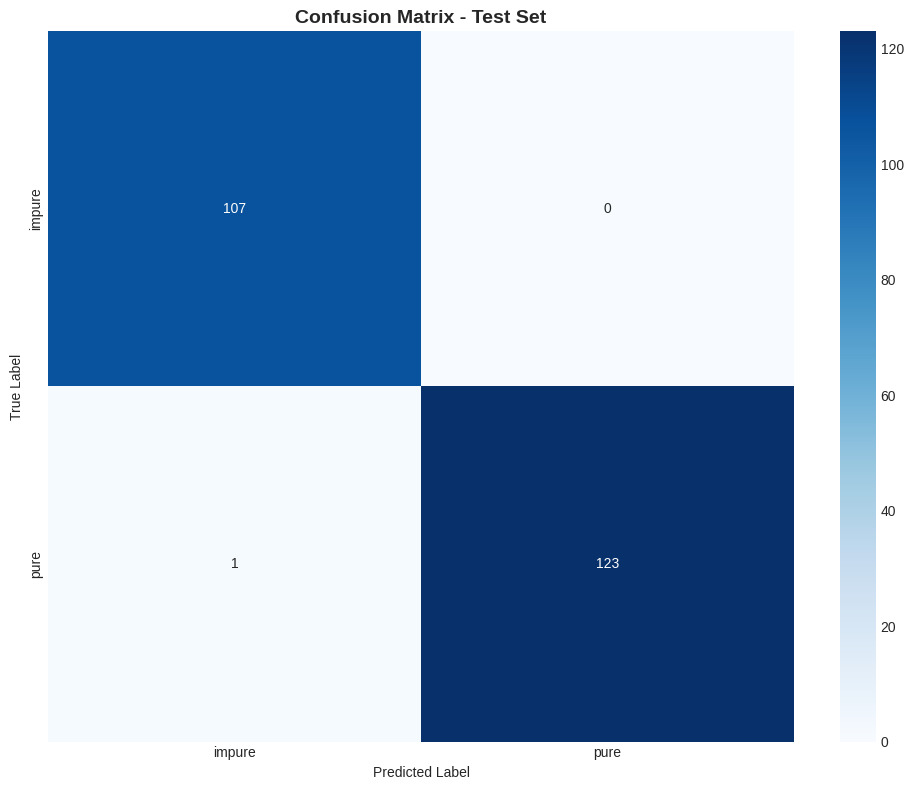
\includegraphics[width=\textwidth]{images/confusion-matrix.jpeg}
  \caption{Visual representation of how often the model got predictions right or wrong.}
  \label{fig:confusion-matrix}
\end{figure}

Out of the 231 test samples evaluated, the model correctly classified 230 samples. The specific classification outcomes are analyzed below:

\textbf{Impure Class (107 Samples):} All 107 impure samples were correctly classified as impure (True Positives), yielding zero false negatives. From an agricultural safety perspective, this prevents the inadvertent distribution and planting of defective or counterfeit seed batches.

\textbf{Pure Class (124 Samples):} The model correctly identified 123 pure samples (True Negatives), with only 1 sample misclassified as impure (False Positive). This conservative error is preferable in agricultural workflows; while a false positive merely necessitates a secondary manual inspection, a false negative (failing to identify impure seeds) could lead to complete crop failure and economic losses for the farmer.

\section{Regularization Effectiveness}

With a dataset size of 1,563 images, training deep neural networks introduces a significant risk of overfitting, where the model memorizes high-frequency noise in the training set rather than extracting generalizable morphological features. To mitigate this, several regularization techniques were evaluated, as compared in Table~\ref{tab:regularization}.

\begin{table}[htbp]
  \centering
  \caption{How Our Anti-Overfitting Techniques Helped}
  \label{tab:regularization}
  \small
  \renewcommand{\arraystretch}{1.1}
  \begin{tabularx}{\textwidth}{|p{4.2cm}|p{4.8cm}|X|}
    \hline
    \textbf{Configuration} & \textbf{Train vs. Validation Gap} & \textbf{What Happened} \\
    \hline
    No Protection & 25--30\% & Bad---the model memorized training data and performed much worse on new seeds \\
    \hline
    Dropout Only & 8--12\% & Better, but still some overfitting on tricky seed textures \\
    \hline
    All Techniques Combined & 2.8\% & Excellent---tight control with less than 5\% difference \\
    \hline
  \end{tabularx}
\end{table}

The validation-to-training accuracy gap was reduced to 2.8\% when all regularization methods were active. This small generalization error indicates that the network successfully extracted generalizable features. This was achieved through the following architectural and optimization strategies:

\begin{itemize}
    \item \textbf{Weight Decay (AdamW):} L2 regularization was applied to penalize large weight magnitudes, thereby constraining model complexity and improving generalization~\cite{loshchilov2019adamw}.
    
    \item \textbf{Label Smoothing:} Soft targets were introduced during cross-entropy loss computation to prevent the model from outputting overconfident logit predictions, which enhances calibration~\cite{muller2019label}.
    
    \item \textbf{Dropout and Batch Normalization:} A dropout rate of 0.5 was applied to the fully connected layers to prevent co-adaptation of features, while batch normalization was utilized to stabilize internal covariate shift~\cite{he2016deep}.
    
    \item \textbf{Learning Rate Scheduling:} A cosine annealing scheduler was implemented to dynamically decay the learning rate, allowing the optimizer to navigate complex loss landscapes and converge to flatter local minima.
    
    \item \textbf{Data Augmentation:} Diverse geometric and photometric transformations---including rotation, flipping, Gaussian blurring, and color jittering---were applied to simulate environmental variations encountered during field photography.
\end{itemize}

\section{Model Comparison and Architecture Selection}

Prior to selecting ResNet50 as the primary backbone, a comparative analysis was conducted using four prominent convolutional neural network architectures trained under identical hyperparameters and optimization settings. The quantitative evaluation metrics are compiled in Table~\ref{tab:modelcomparison}, and the trade-off between classification accuracy and training computational overhead is illustrated in Figure~\ref{fig:model-comparison}.

\begin{table}[htbp]
  \centering
  \caption{Comparing Four Different Neural Network Architectures}
  \label{tab:modelcomparison}
  \small
  \renewcommand{\arraystretch}{1.1}
  \begin{tabularx}{\textwidth}{|p{3.2cm}|c|c|c|c|X|}
    \hline
    \textbf{Model} & \textbf{Accuracy} & \textbf{Precision} & \textbf{Recall} & \textbf{F1 Score} & \textbf{Training Time} \\
    \hline
    \textbf{ResNet50} & \textbf{99.57\%} & \textbf{99.57\%} & \textbf{99.57\%} & \textbf{99.57\%} & 16.4 min \\
    \hline
    \textbf{DenseNet121} & 99.57\% & 99.57\% & 99.57\% & \textbf{99.57\%} & 15.0 min \\
    \hline
    \textbf{GoogleNet} & 99.57\% & 99.57\% & 99.57\% & \textbf{99.57\%} & 12.2 min \\
    \hline
    \textbf{MobileNetV2} & 99.13\% & 99.15\% & 99.13\% & 99.13\% & \textbf{8.5 min} \\
    \hline
  \end{tabularx}
\end{table}

\begin{figure}[htbp]
  \centering
  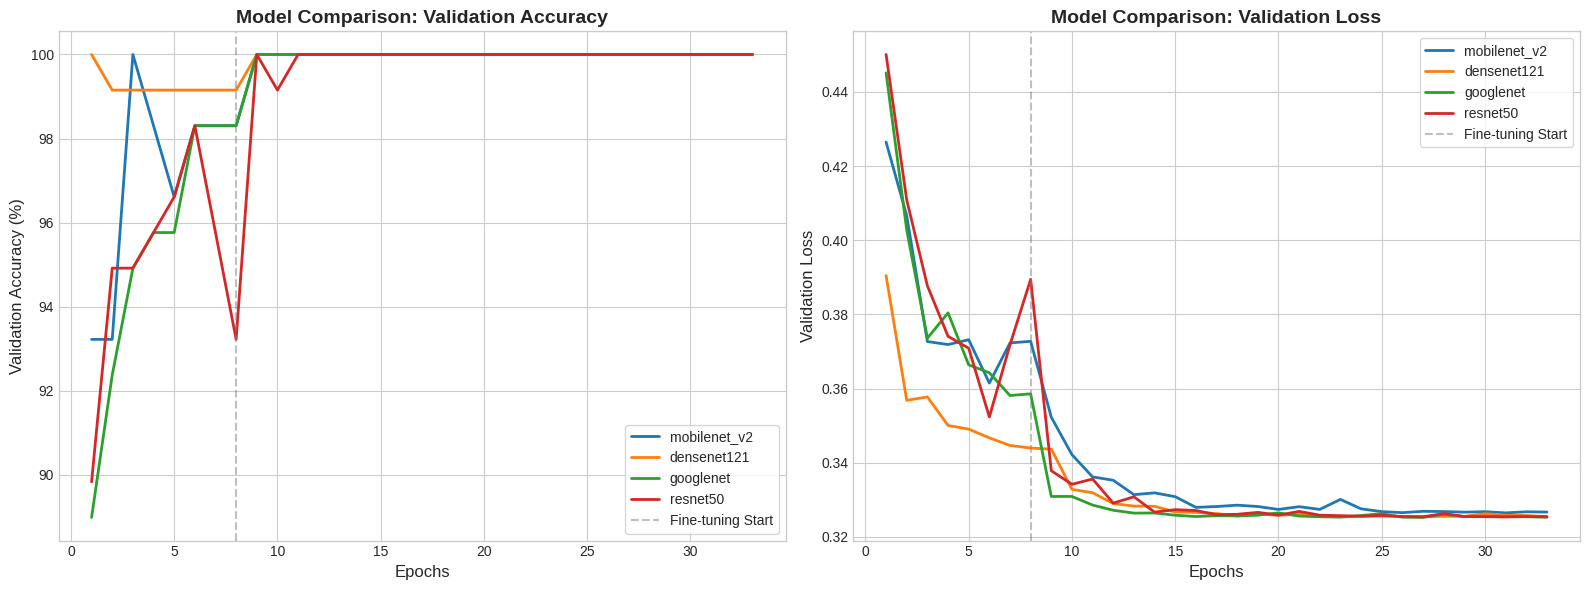
\includegraphics[width=\textwidth]{images/model-comparison.jpeg}
  \caption{Visual comparison of how each model performed and how long training took.}
  \label{fig:model-comparison}
\end{figure}

ResNet50, DenseNet121, and GoogLeNet achieved identical classification accuracies of 99.57\%. MobileNetV2 registered a slightly lower accuracy of 99.13\% but required significantly less training time. ResNet50 was selected as the final architecture due to several specific advantages.

The residual connections (skip connections) in ResNet50 address the vanishing gradient problem, allowing efficient backpropagation through the 50-layer architecture and facilitating fine-tuning without information loss~\cite{he2016deep, xu2021}. Furthermore, ResNet50 exhibits superior compatibility across deployment frameworks, including PyTorch, TorchScript, ONNX, and edge-optimized runtime engines. This cross-platform compatibility supports future plans to deploy AgriVerify as a native mobile application. The marginal training time overhead (an additional 4.4 minutes compared to GoogLeNet) is offset by these deployment advantages, given that model training is an offline process~\cite{pytorch2019}.

\section{System Performance and Production Latency}

In addition to classification accuracy, computational efficiency and response latency are critical parameters for real-time applications deployed in agricultural fields.

\subsection{Inference Latency Evaluation}

Model inference latency refers to the duration required for the network to ingest a preprocessed image, perform a forward pass, and output the class probabilities. The latency profiles across different hardware configurations are summarized in Table~\ref{tab:latency}.

\begin{table}[htbp]
  \centering
  \caption{Speed on Different Hardware}
  \label{tab:latency}
  \small
  \renewcommand{\arraystretch}{1.1}
  \begin{tabularx}{\textwidth}{|p{4.5cm}|c|X|}
    \hline
    \textbf{Hardware} & \textbf{Speed} & \textbf{Good For What?} \\
    \hline
    Regular CPU & $\sim$165 ms & Lightweight servers and edge devices; still plenty fast \\
    \hline
    GPU (NVIDIA CUDA) & $\sim$20 ms & Cloud servers handling many requests; 8 times faster than CPU \\
    \hline
  \end{tabularx}
\end{table}

On standard CPU architectures (without hardware acceleration), the model achieved an average inference latency of approximately 165 ms. When evaluated on GPU hardware (NVIDIA CUDA), the latency was reduced to 20 ms. Both execution speeds are well within acceptable thresholds for interactive, real-time application feedback.

\subsection{End-to-End System Performance Under Load}

To evaluate the scalability of the backend system under high concurrent access conditions, stress testing was conducted. The system throughput and latency metrics under simulated concurrent loads are detailed in Table~\ref{tab:backendperformance}.

\begin{table}[htbp]
  \centering
  \caption{Real-World System Performance Under Load}
  \label{tab:backendperformance}
  \small
  \renewcommand{\arraystretch}{1.1}
  \begin{tabularx}{\textwidth}{|p{4.5cm}|c|X|}
    \hline
    \textbf{Metric} & \textbf{Observation} & \textbf{Significance} \\
    \hline
    End-to-End Response & 280--420 ms & Includes uploading the image, sending it through the system, running AI, and formatting the response \\
    \hline
    Concurrent Requests & 40--60 per second & Very stable even when many farmers submit seeds simultaneously \\
    \hline
    Image Upload \& Prep & 80--120 ms & Network transfer and image preprocessing before AI runs \\
    \hline
    Database Queries & $<$50 ms & Fast retrieval of complaint and user records \\
    \hline
  \end{tabularx}
\end{table}

The system demonstrated high stability and responsiveness under peak concurrent loads. The asynchronous proxy design pattern prevents thread blocking at the core application layer by managing intensive operations outside the main request-response cycle, thereby preserving database and API availability~\cite{martin2018clean}.

\section{Functional Verification and Test Execution}

System validation was conducted to verify functional correctness, security enforcement, and data integrity across all primary operational workflows.

\subsection{Seed Classification Subsystem Validation}

The image processing pipeline and classification subsystem were validated against diverse input scenarios. The specific test cases, expected behaviors, and execution results are detailed in Table~\ref{tab:seedtestcases}.

\begin{table}[htbp]
  \centering
  \caption{Seed Verification Test Cases}
  \label{tab:seedtestcases}
  \small
  \renewcommand{\arraystretch}{1.1}
  \begin{tabularx}{\textwidth}{|p{1.6cm}|X|X|c|}
    \hline
    \textbf{Test ID} & \textbf{What We Tested} & \textbf{Expected Behavior} & \textbf{Result} \\
    \hline
    \textbf{SV-01} & Upload clear photos of genuine seed packaging & Correctly classified as Pure with physical measurements extracted & \textbf{Pass} \\
    \hline
    \textbf{SV-02} & Upload photos of cracked or discolored seeds & Classified as Impure (Damaged) with warnings shown & \textbf{Pass} \\
    \hline
    \textbf{SV-03} & Upload fake packaging with counterfeit branding & Classified as Impure (Fake) with high confidence & \textbf{Pass} \\
    \hline
    \textbf{SV-04} & Try uploading wrong file types (.exe, .zip, .txt) & System rejects and shows helpful error message & \textbf{Pass} \\
    \hline
    \textbf{SV-05} & Upload blurry or very dark seed photos & System warns user to retake photo or shows low confidence & \textbf{Pass} \\
    \hline
  \end{tabularx}
\end{table}

\subsection{Grievance Management Subsystem Validation}

The complaint lodging and tracking functionalities were validated to verify database consistency and transactional security. The validation test cases are outlined in Table~\ref{tab:complainttestcases}.

\begin{table}[htbp]
  \centering
  \caption{Complaint System Test Cases}
  \label{tab:complainttestcases}
  \small
  \renewcommand{\arraystretch}{1.1}
  \begin{tabularx}{\textwidth}{|p{1.6cm}|X|X|c|}
    \hline
    \textbf{Test ID} & \textbf{What We Tested} & \textbf{Expected Behavior} & \textbf{Result} \\
    \hline
    \textbf{CM-01} & Farmer files a complaint with description and evidence & Complaint saved to database and marked as Open & \textbf{Pass} \\
    \hline
    \textbf{CM-02} & Try filing complaint with missing required information & Form validation prevents submission and shows error & \textbf{Pass} \\
    \hline
    \textbf{CM-03} & Farmer views their complaint history & All past and current complaints displayed with pagination & \textbf{Pass} \\
    \hline
    \textbf{CM-04} & Officer changes complaint status from Open to Resolved & Update immediately visible in the system & \textbf{Pass} \\
    \hline
  \end{tabularx}
\end{table}

\subsection{Role-Based Access Control and Security Verification}

To ensure secure operations, the authorization and authentication mechanisms were tested against access violations. The results of the security test cases are compiled in Table~\ref{tab:rbactestcases}.

\begin{table}[htbp]
  \centering
  \caption{Security and Access Control Test Cases}
  \label{tab:rbactestcases}
  \small
  \renewcommand{\arraystretch}{1.1}
  \begin{tabularx}{\textwidth}{|p{1.6cm}|X|X|c|}
    \hline
    \textbf{Test ID} & \textbf{What We Tested} & \textbf{Expected Behavior} & \textbf{Result} \\
    \hline
    \textbf{RB-01} & Valid farmer login & Receives security token and goes to farmer dashboard & \textbf{Pass} \\
    \hline
    \textbf{RB-02} & Farmer tries accessing admin page & System blocks access and redirects to farmer area & \textbf{Pass} \\
    \hline
    \textbf{RB-03} & Admin login with multi-factor authentication & Full admin privileges granted & \textbf{Pass} \\
    \hline
    \textbf{RB-04} & Security token expires during session & System automatically gets new token without user noticing & \textbf{Pass} \\
    \hline
    \textbf{RB-05} & Login with wrong password & System returns error and shows helpful message & \textbf{Pass} \\
    \hline
  \end{tabularx}
\end{table}

% ──────────────────────────────────────────────────────────────
\section{System User Interfaces and Operational Workflows}
\label{sec:system-interfaces}
% ──────────────────────────────────────────────────────────────

AgriVerify provides simple, intuitive interfaces tailored to three different user types: farmers, agricultural officers, and system administrators. We built these using modern web technologies: Next.js 15, React 19, and Tailwind CSS~\cite{nextjs2024, react2013, tailwind2024}. Let's walk through each interface and see how users interact with the system.

\subsection{Public Portal, Onboarding, and Multilingual Support}

Upon accessing the AgriVerify platform, users are presented with the public landing page, which outlines the system's value proposition and operational features (Figure~\ref{fig:ui-landing}). To accommodate rural demographics, the platform incorporates a localized language selection interface, enabling users to transition between English and regional dialects (Figure~\ref{fig:ui-language}).

\begin{figure}[htbp]
  \centering
  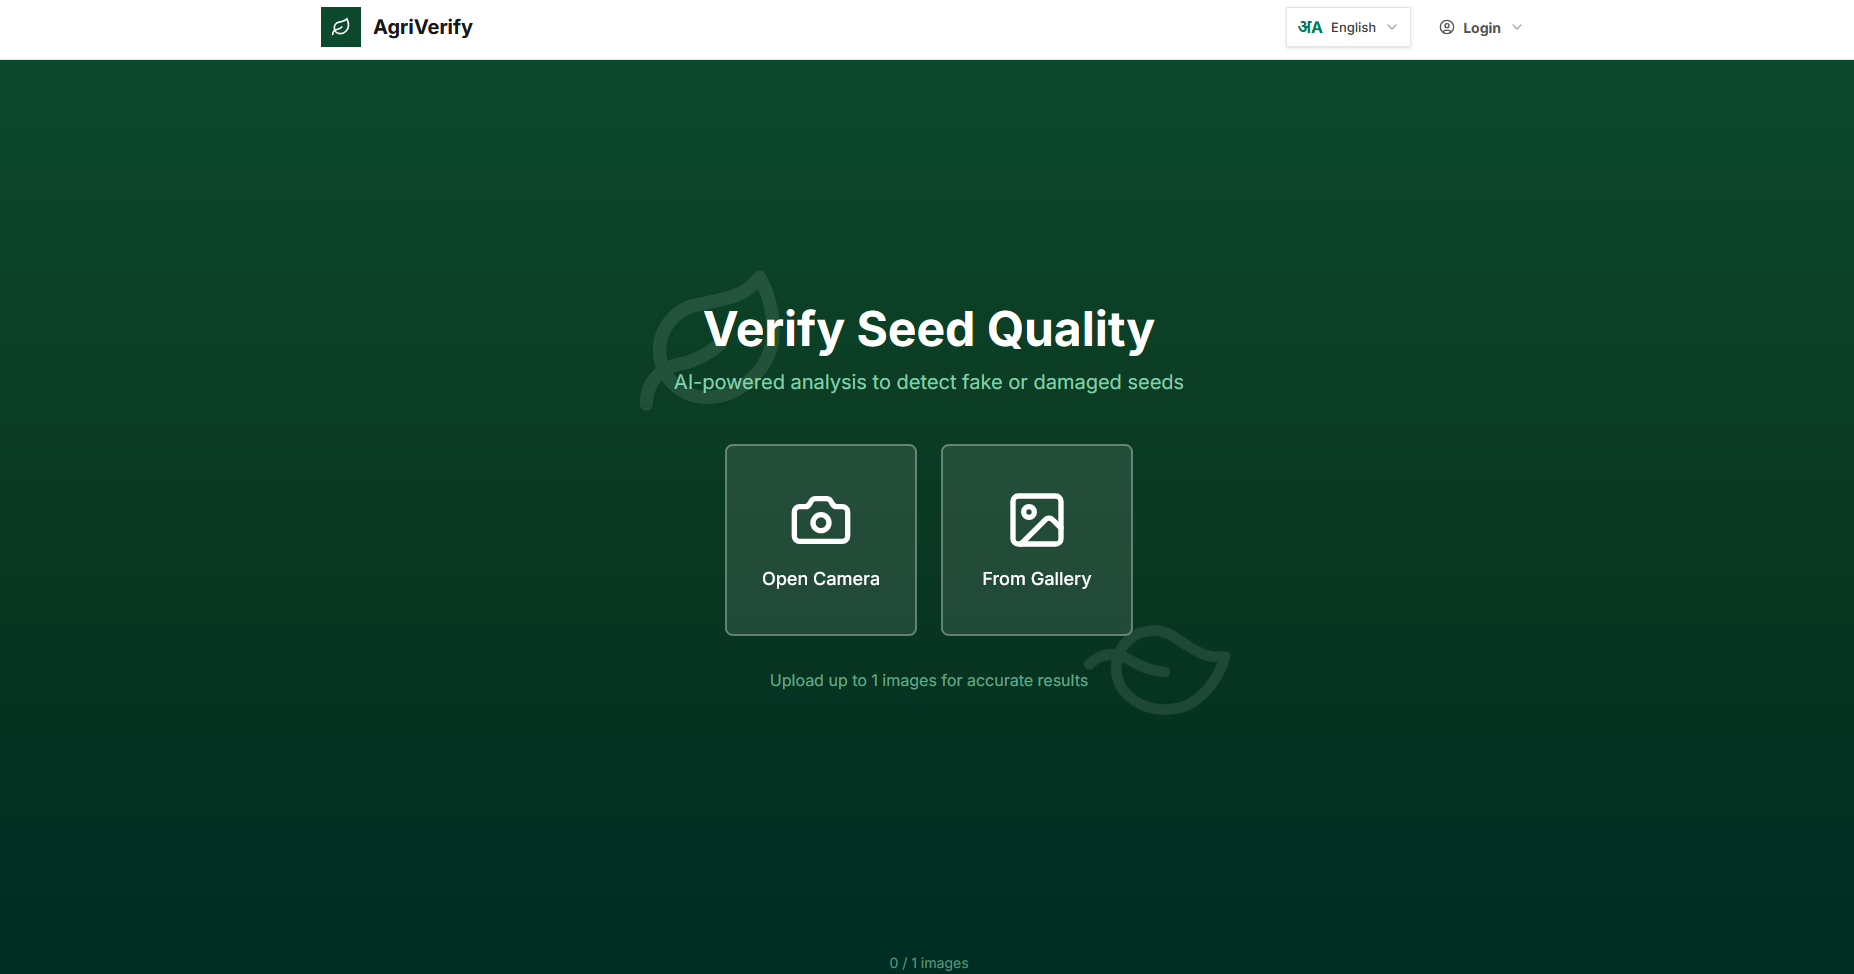
\includegraphics[width=\textwidth]{images/landing.png}
  \caption{Platform landing page displaying value proposition and core features.}
  \label{fig:ui-landing}
\end{figure}

\begin{figure}[htbp]
  \centering
  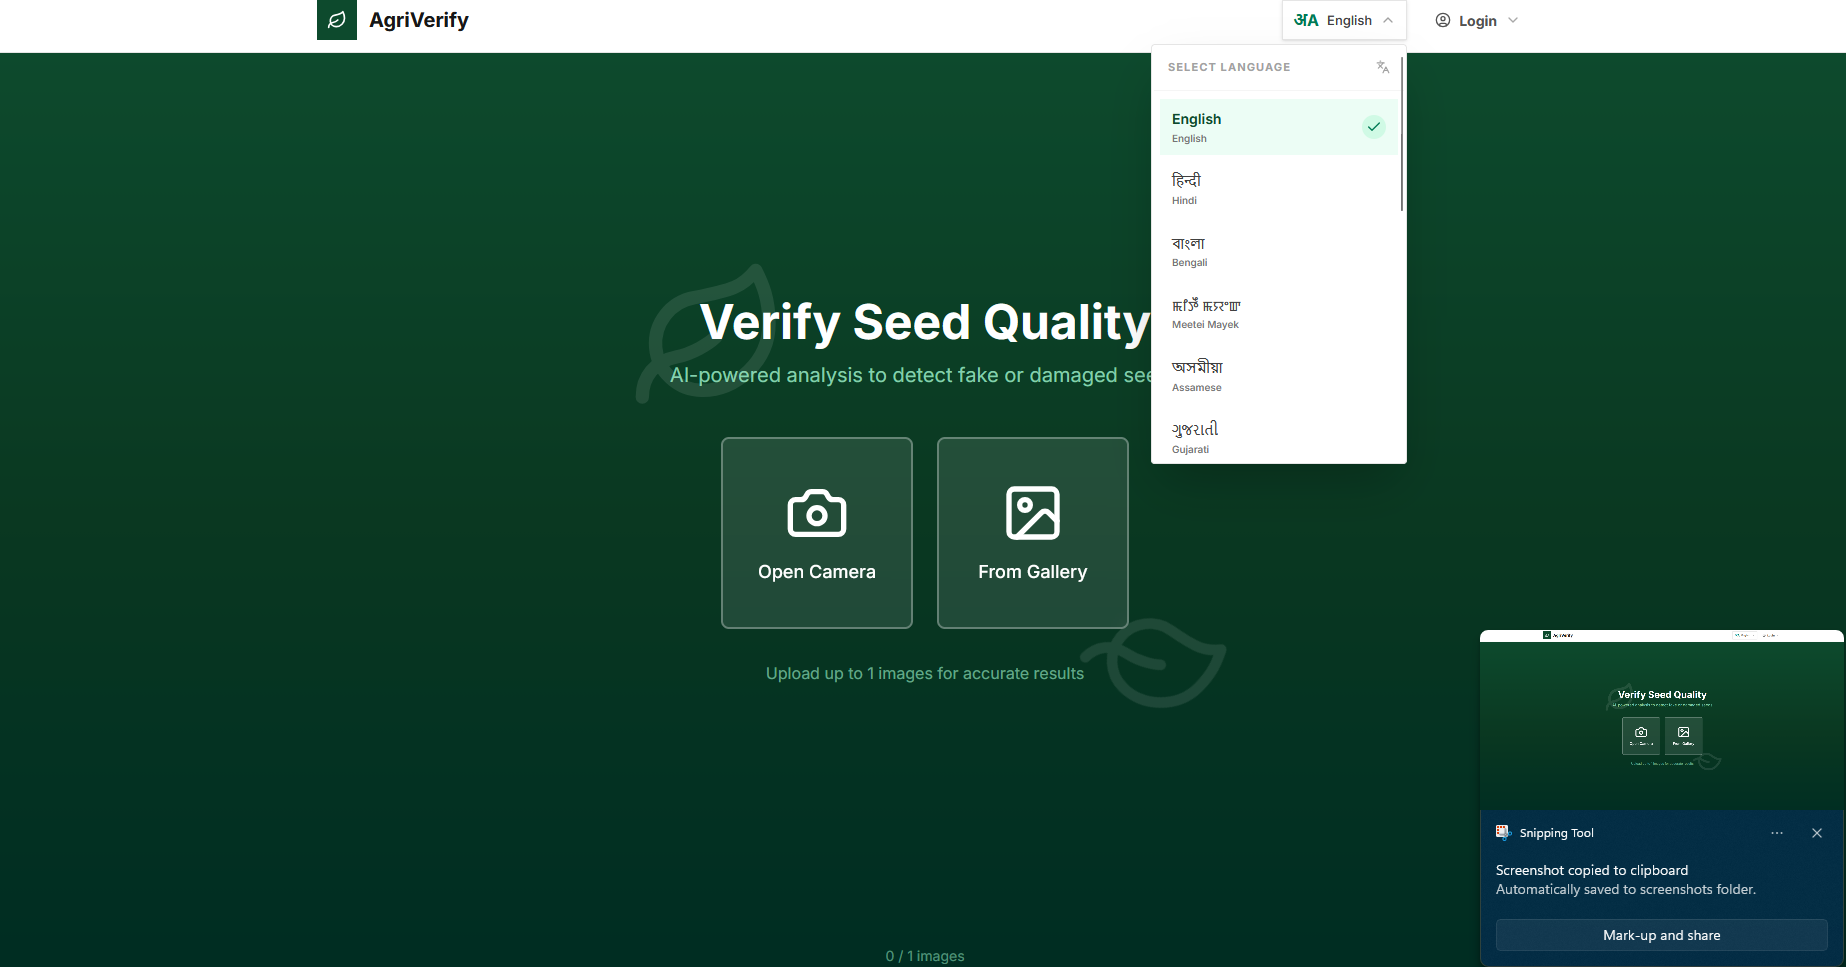
\includegraphics[width=\textwidth]{images/language.png}
  \caption{Multilingual selection interface supporting regional languages.}
  \label{fig:ui-language}
\end{figure}

New users can register by selecting their role (Figure~\ref{fig:ui-login-landing}) and completing the onboarding registration form, which captures demographic, location, and agricultural district details (Figure~\ref{fig:ui-new-account}). This location data is critical for geo-tagging and regional analytics in the grievance management system.

\begin{figure}[htbp]
  \centering
  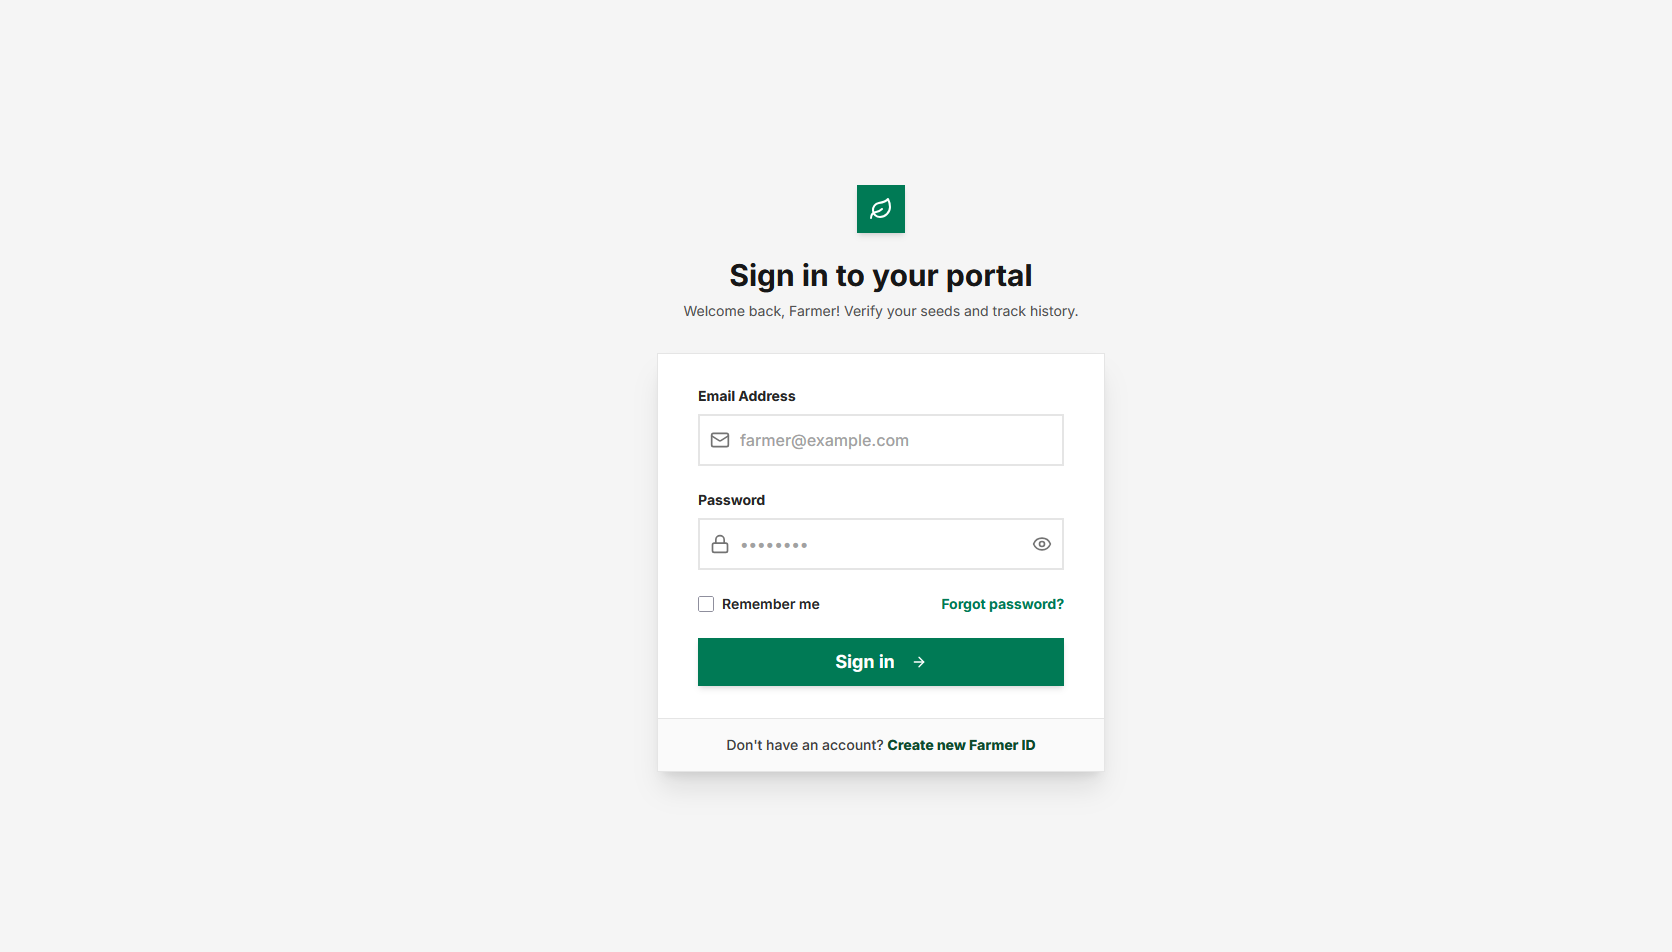
\includegraphics[width=\textwidth]{images/login-landing.png}
  \caption{Role selection interface for login.}
  \label{fig:ui-login-landing}
\end{figure}

\begin{figure}[htbp]
  \centering
  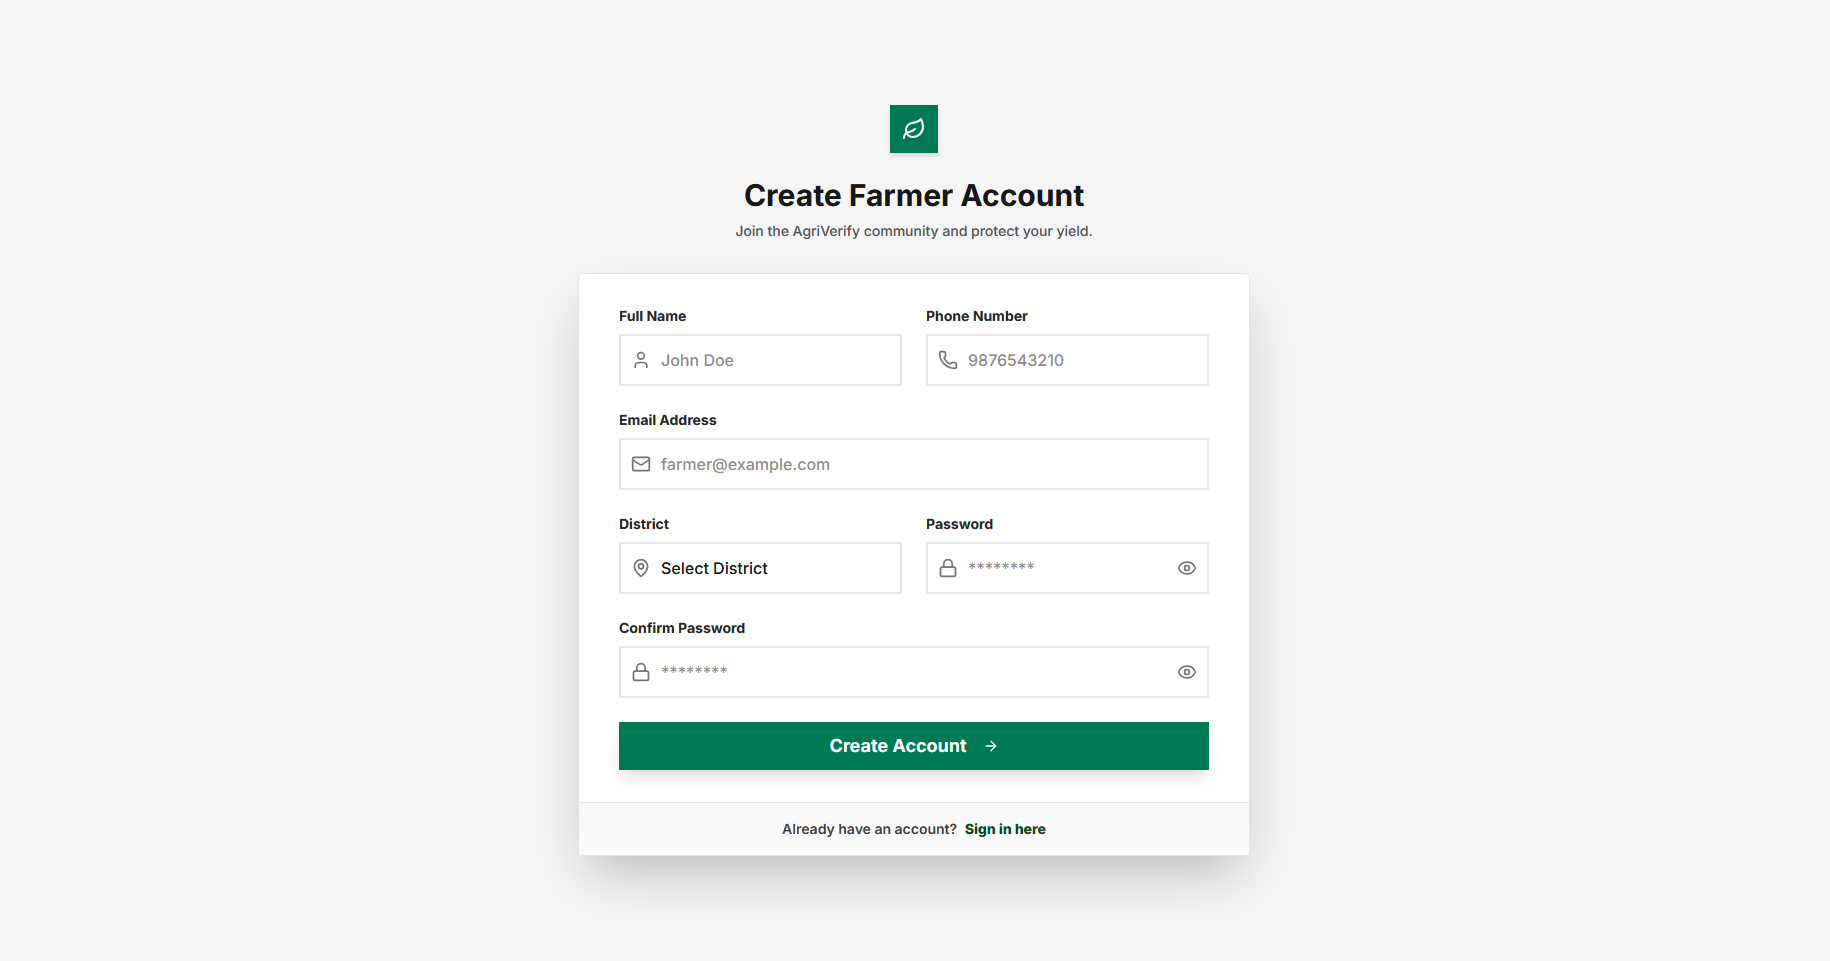
\includegraphics[width=\textwidth]{images/new-account.png}
  \caption{Farmer registration form collecting demographic and location information.}
  \label{fig:ui-new-account}
\end{figure}

For administrative personnel and agricultural officers, a secure portal interface enforces multi-factor authentication (MFA) via time-based security codes to prevent unauthorized administrative actions (Figure~\ref{fig:ui-admin-login}).

\begin{figure}[htbp]
  \centering
  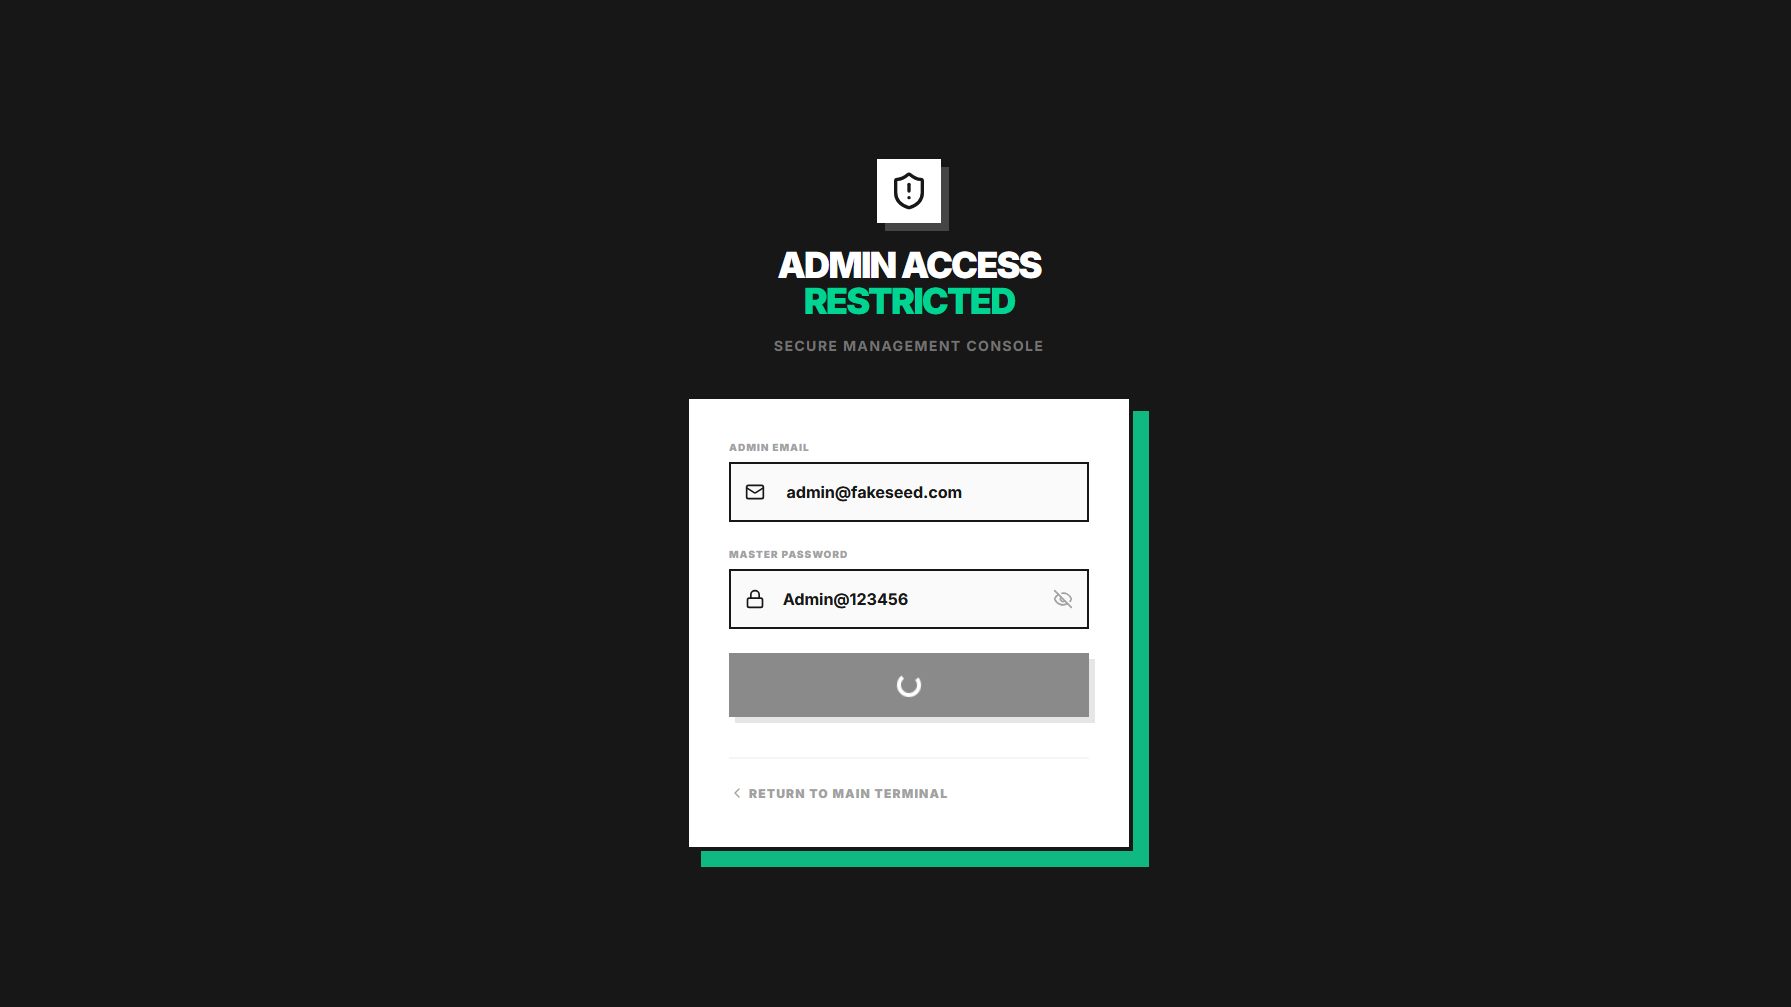
\includegraphics[width=\textwidth]{images/admin-login.png}
  \caption{Secure admin login requiring multi-factor authentication.}
  \label{fig:ui-admin-login}
\end{figure}

\subsection{Farmer Portal and AI Seed Quality Assessment Workflow}

Once authenticated, farmers are redirected to a personalized dashboard containing historical verification records, analytical statistics, and regional agricultural alerts (Figure~\ref{fig:ui-dashboard}). Profile parameters and verification badges can be managed within the user profile interface (Figure~\ref{fig:ui-profile}).

\begin{figure}[htbp]
  \centering
  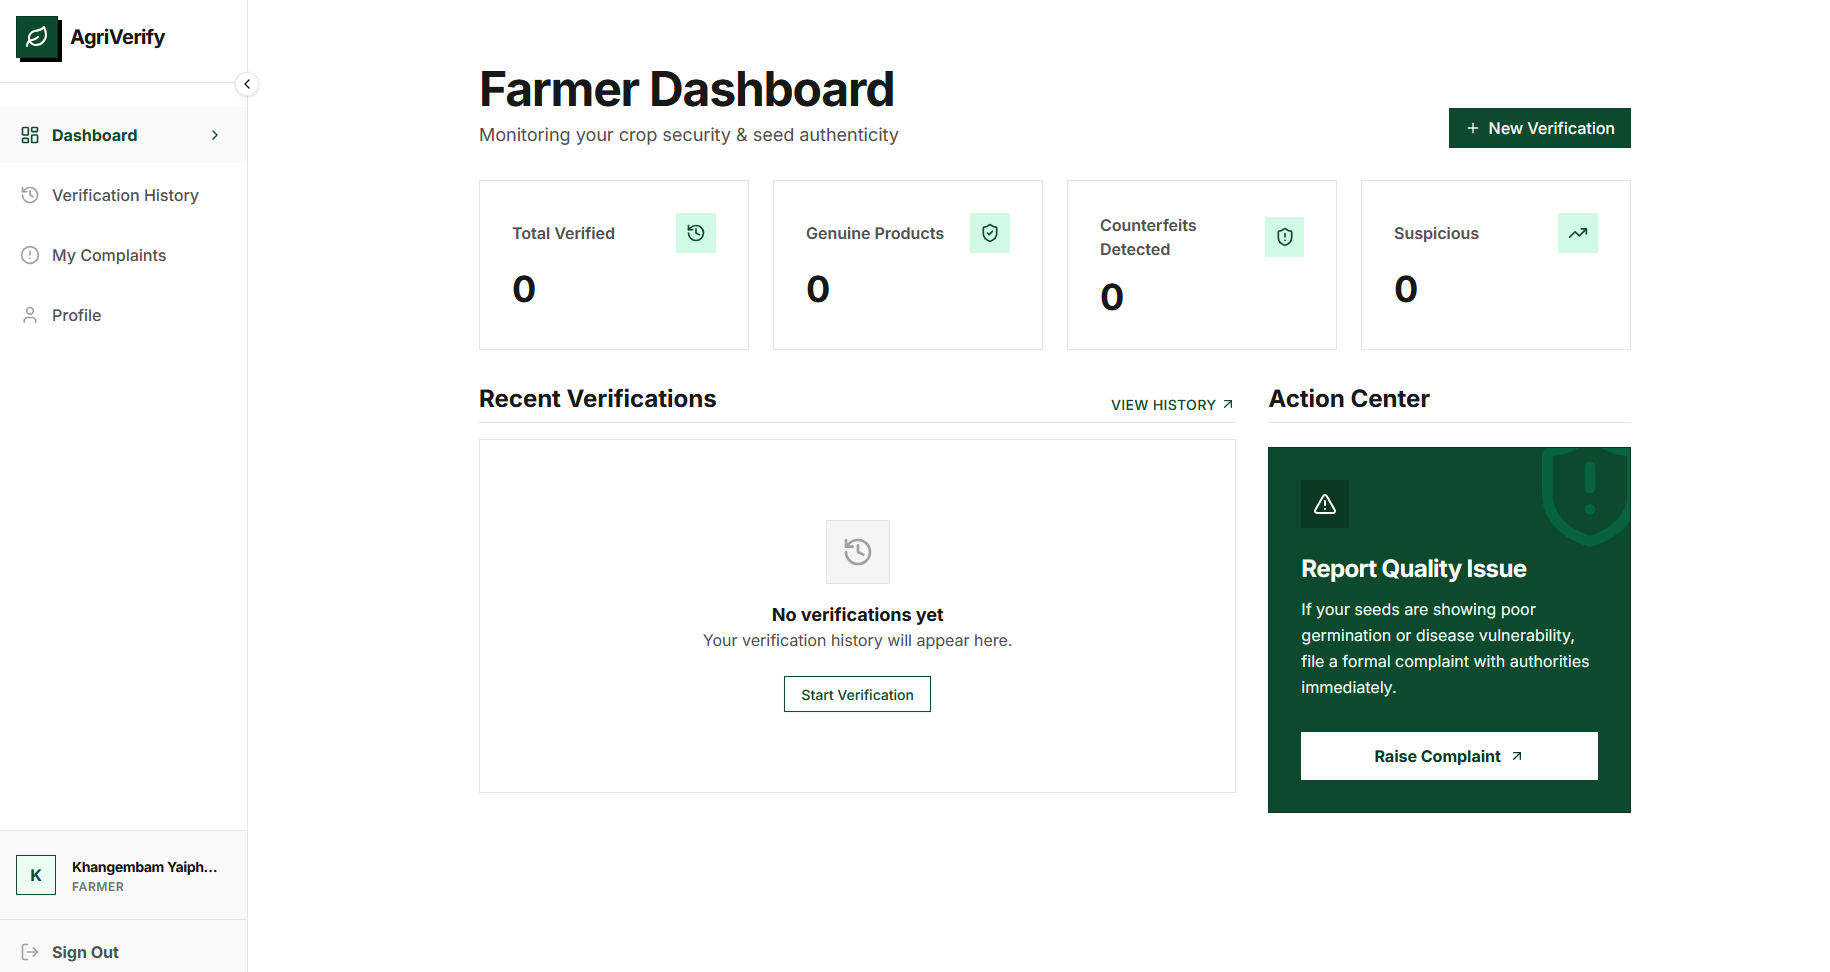
\includegraphics[width=\textwidth]{images/dashboard.png}
  \caption{Farmer dashboard interface displaying verification statistics and history.}
  \label{fig:ui-dashboard}
\end{figure}

\begin{figure}[htbp]
  \centering
  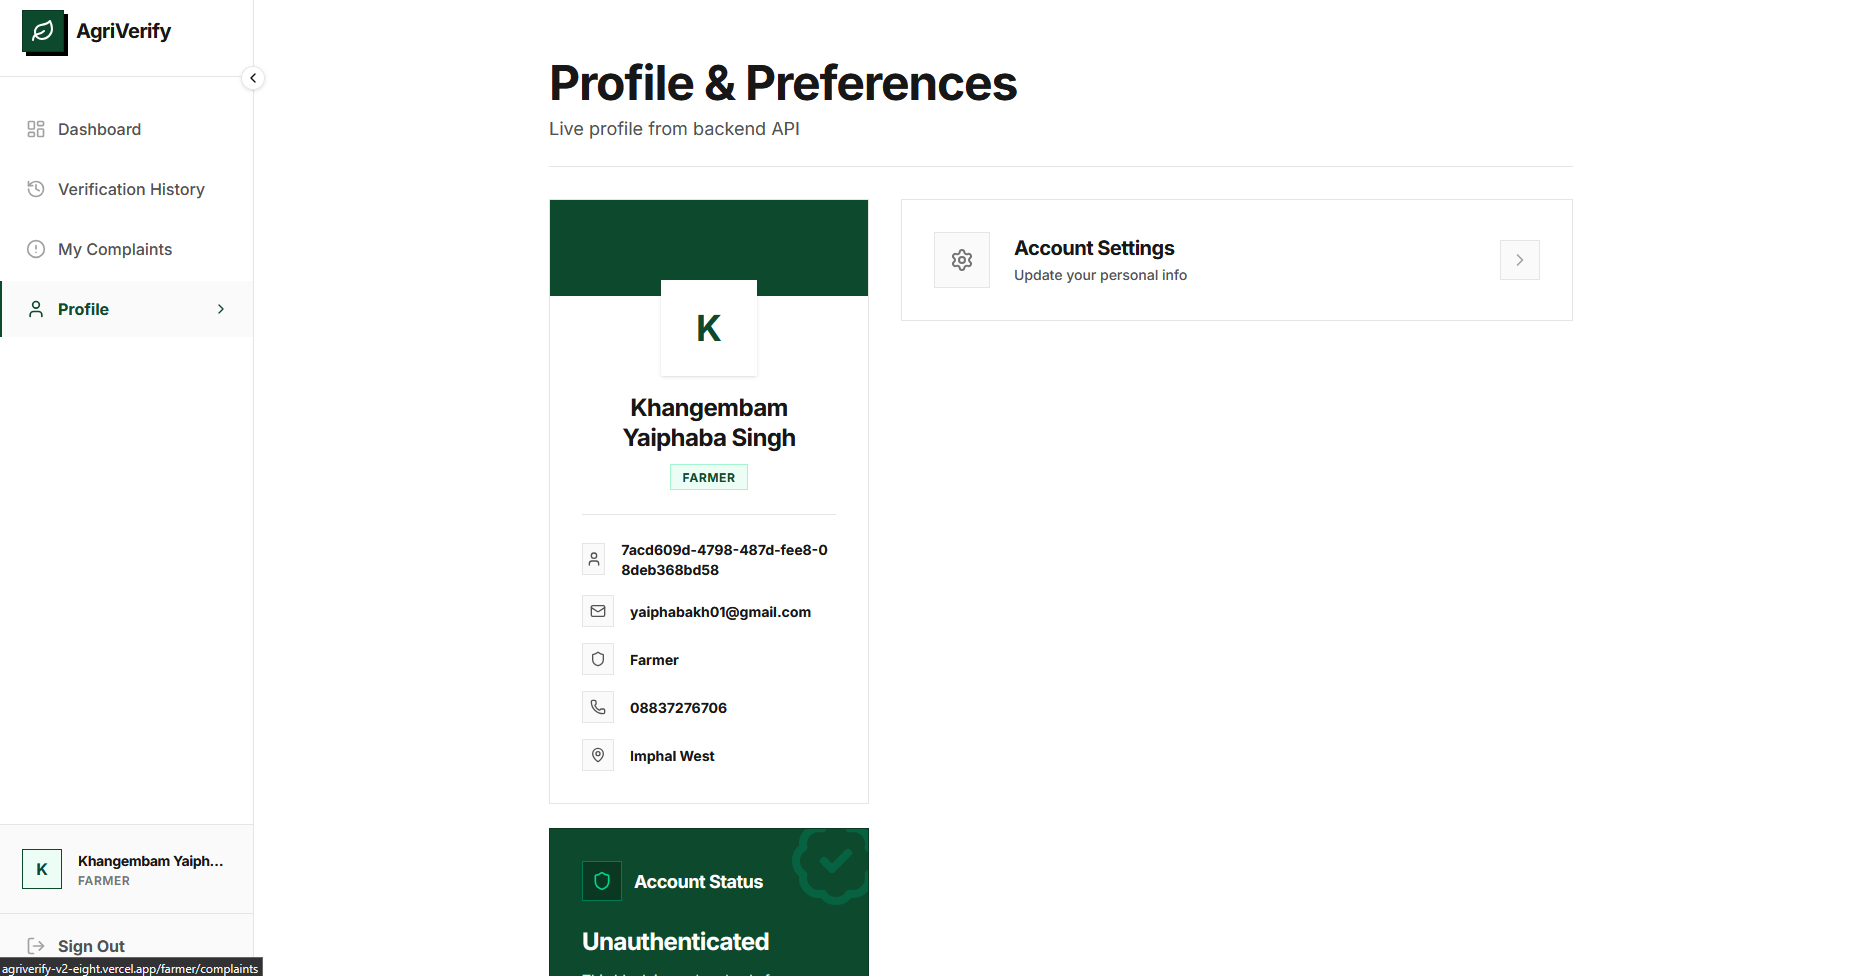
\includegraphics[width=\textwidth]{images/profile.png}
  \caption{Farmer profile configuration interface with verification achievements.}
  \label{fig:ui-profile}
\end{figure}

User details can be modified via the profile configuration interface (Figure~\ref{fig:ui-rename}). The seed assessment workflow is initiated by capturing and submitting high-resolution images of the front and back of the seed packaging using the mobile-optimized camera capture interface (Figure~\ref{fig:ui-adding-seed}).

\begin{figure}[htbp]
  \centering
  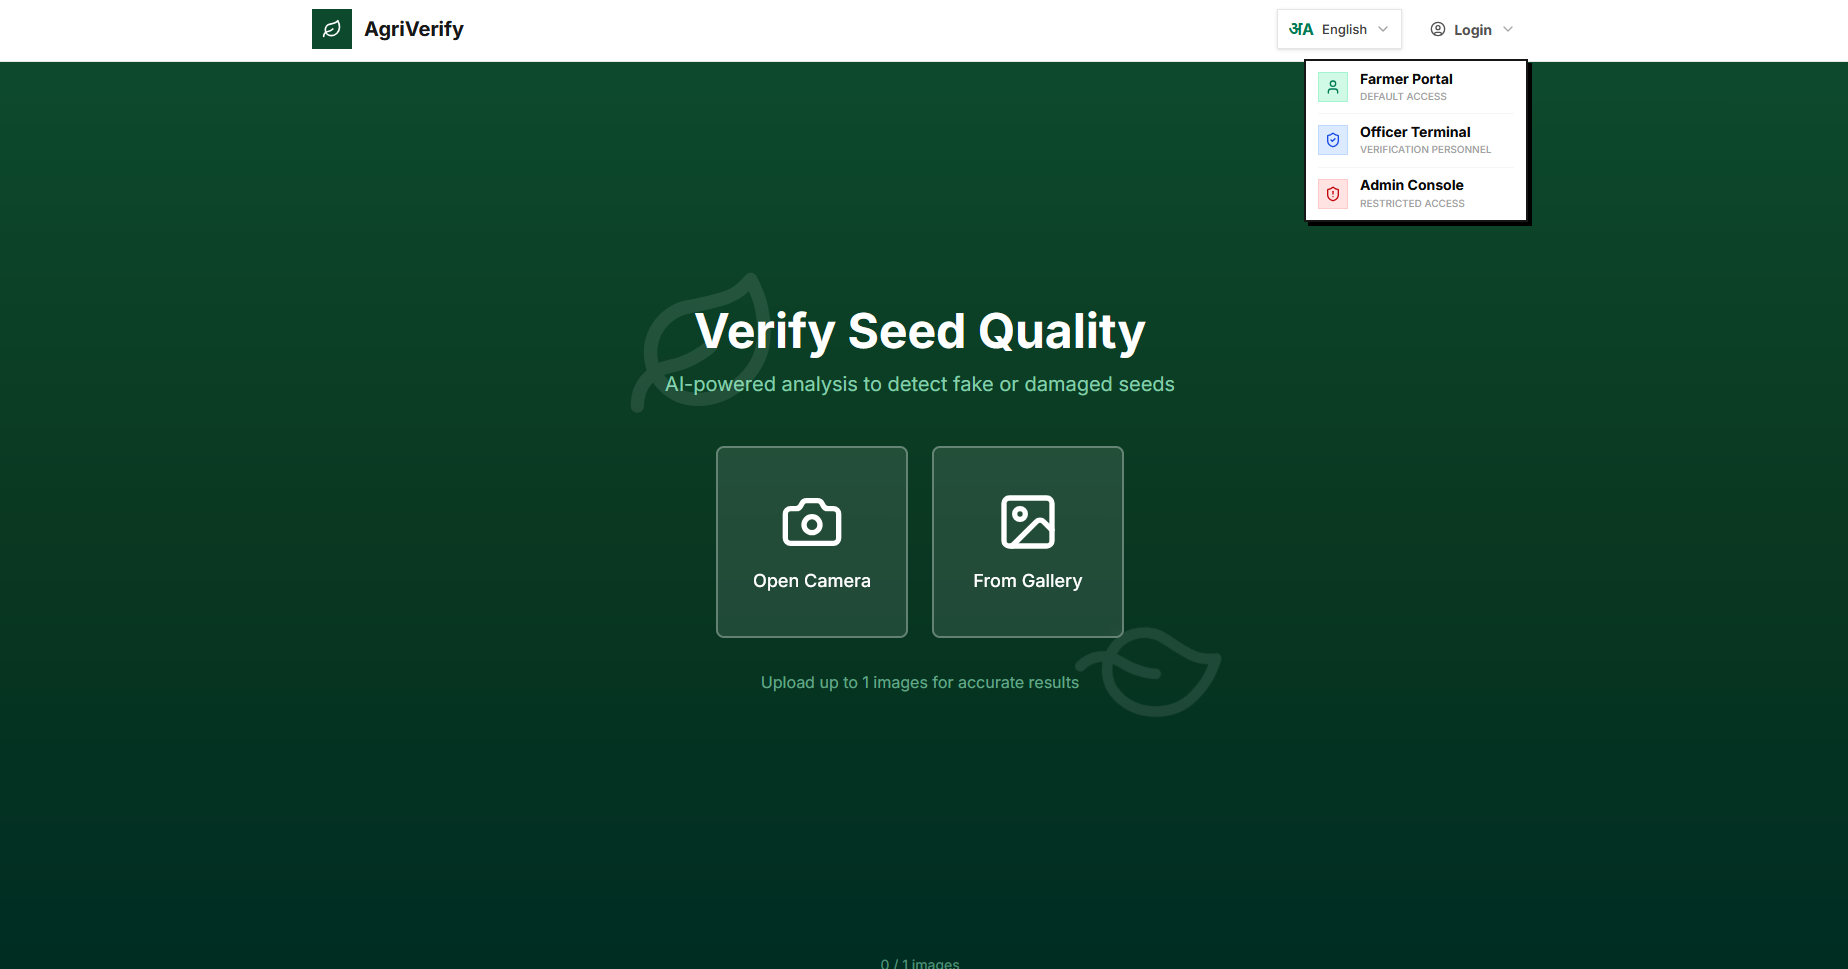
\includegraphics[width=\textwidth]{images/rename.png}
  \caption{User profile modification interface.}
  \label{fig:ui-rename}
\end{figure}

\begin{figure}[htbp]
  \centering
  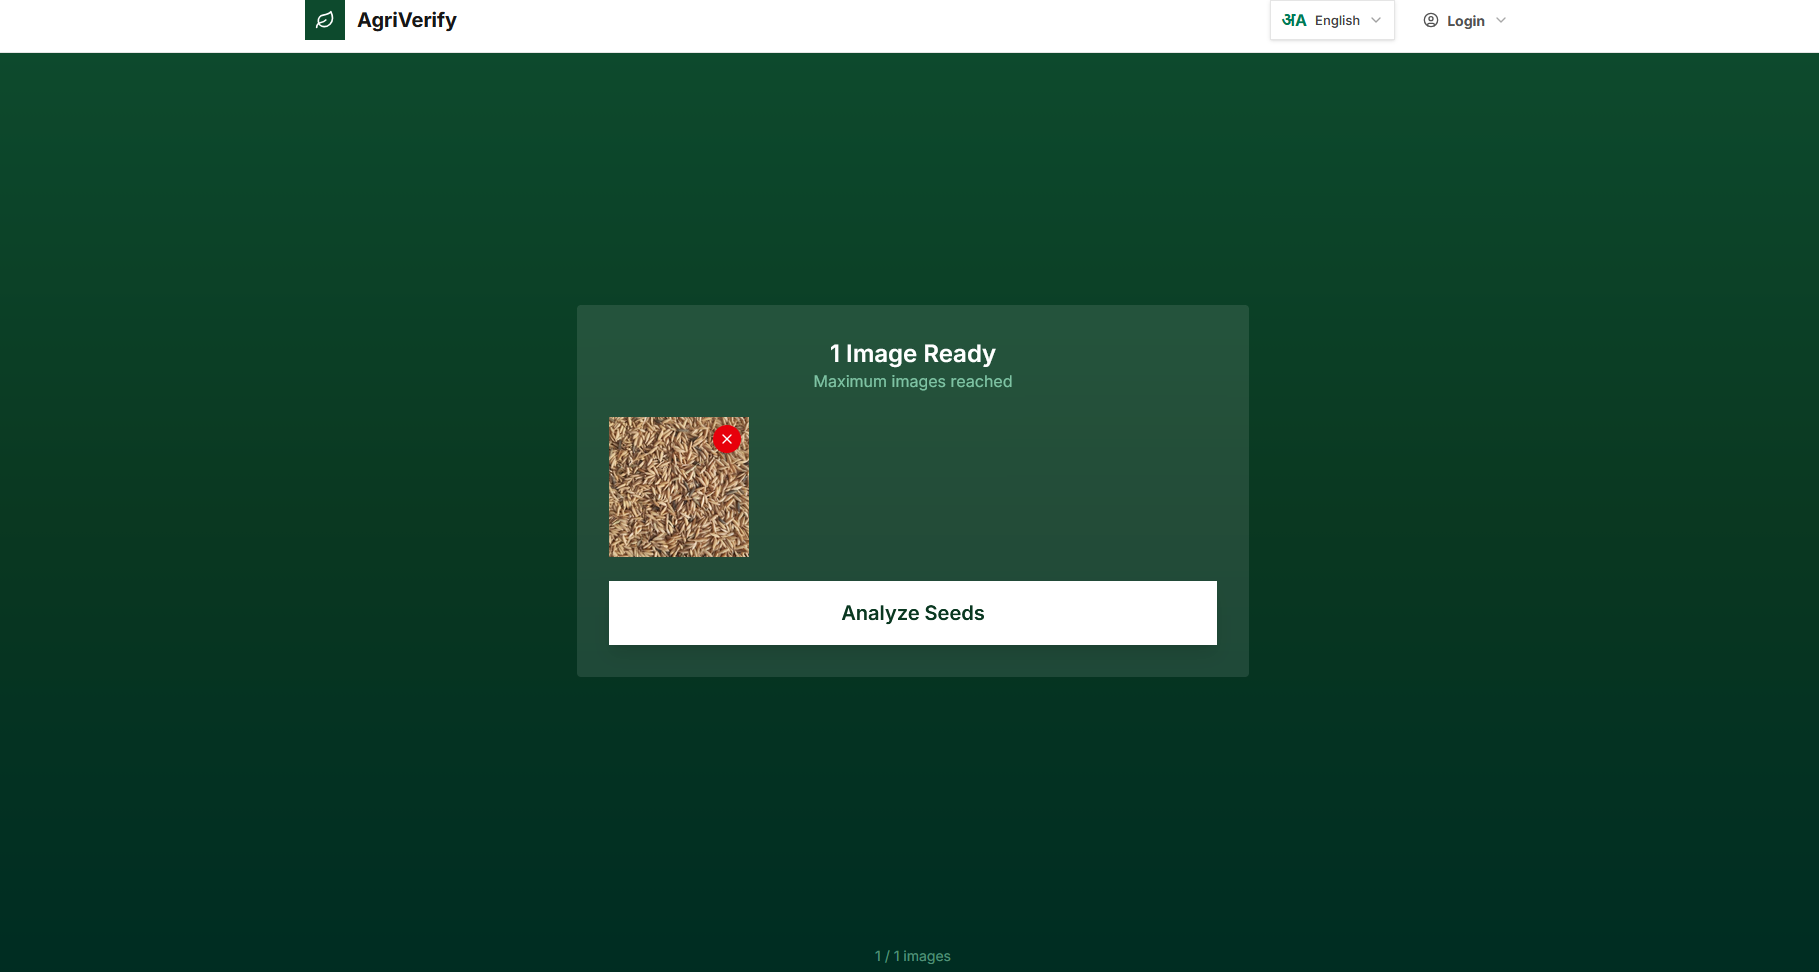
\includegraphics[width=\textwidth]{images/adding-seed-image.png}
  \caption{Mobile camera interface for uploading seed packaging images.}
  \label{fig:ui-adding-seed}
\end{figure}

Following image processing, the model generates a comprehensive quality report. If the seed batch is certified as pure, the interface displays extracted physical characteristics and purity metrics (Figure~\ref{fig:ui-genuine}). Conversely, if defects or counterfeit markers are detected, a warning interface highlights classification confidence and offers remedial instructions (Figure~\ref{fig:ui-counterfeit}).

\begin{figure}[htbp]
  \centering
  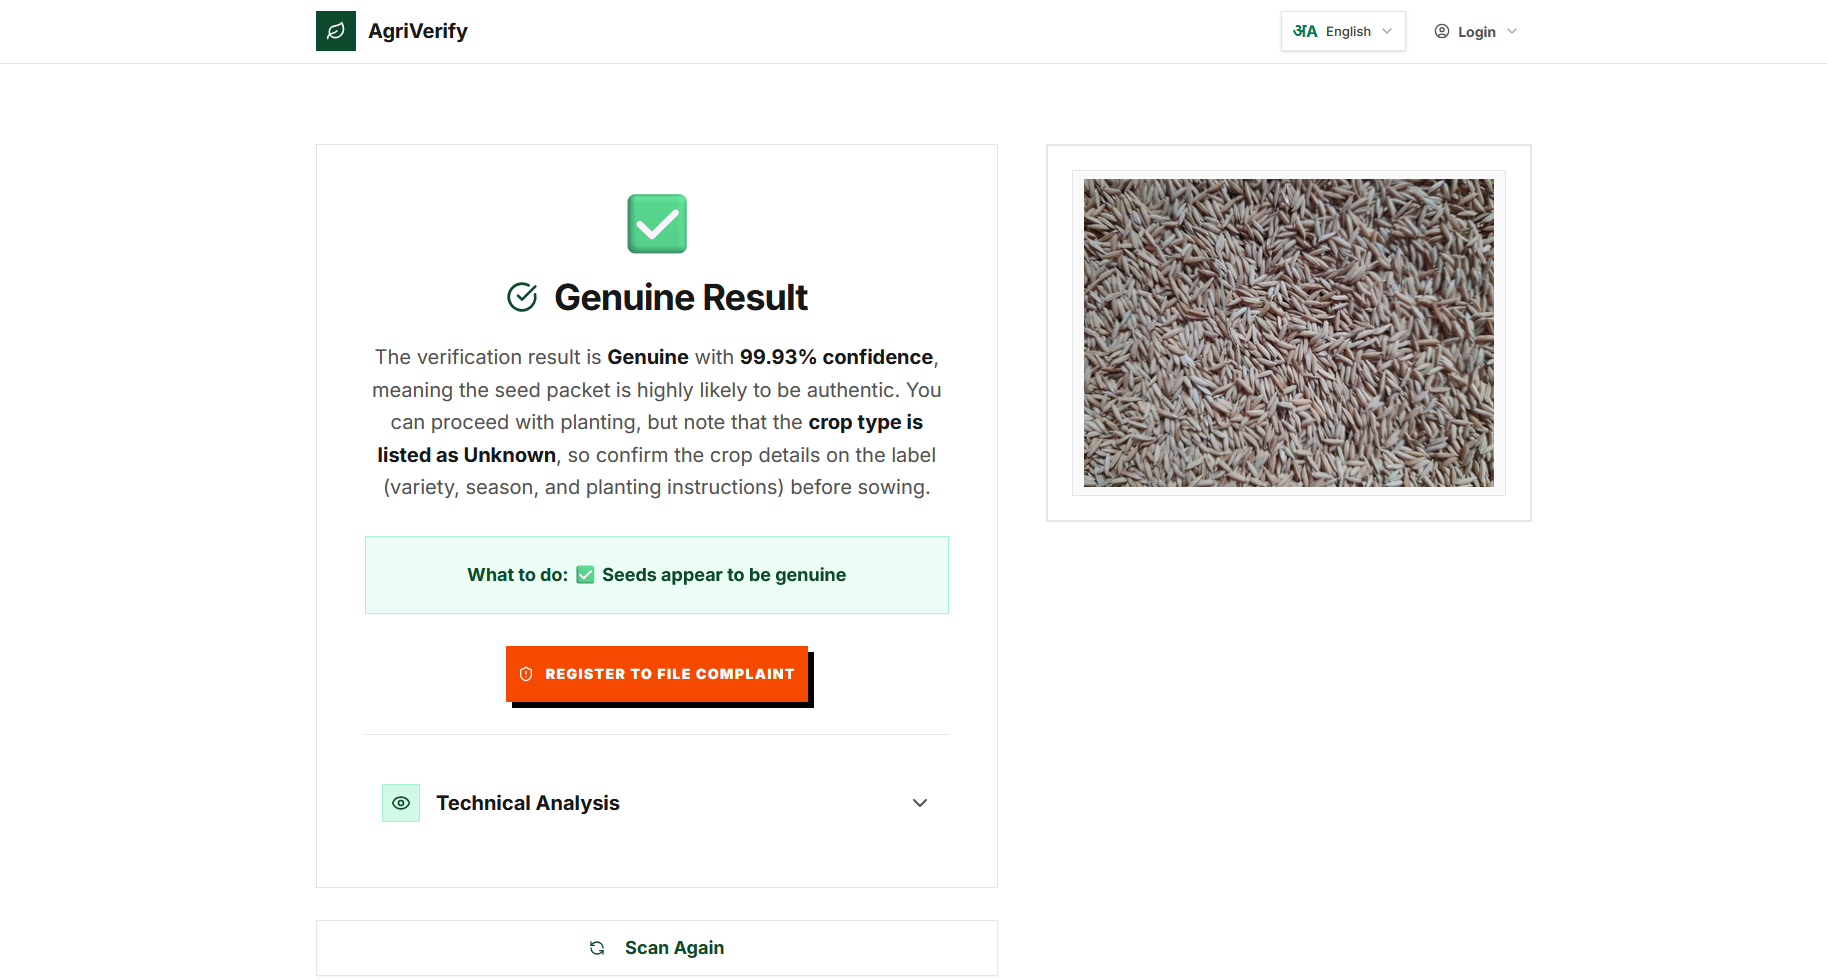
\includegraphics[width=\textwidth]{images/genuine.png}
  \caption{Verification result indicating pure seed batch with morphological measurements.}
  \label{fig:ui-genuine}
\end{figure}

\begin{figure}[htbp]
  \centering
  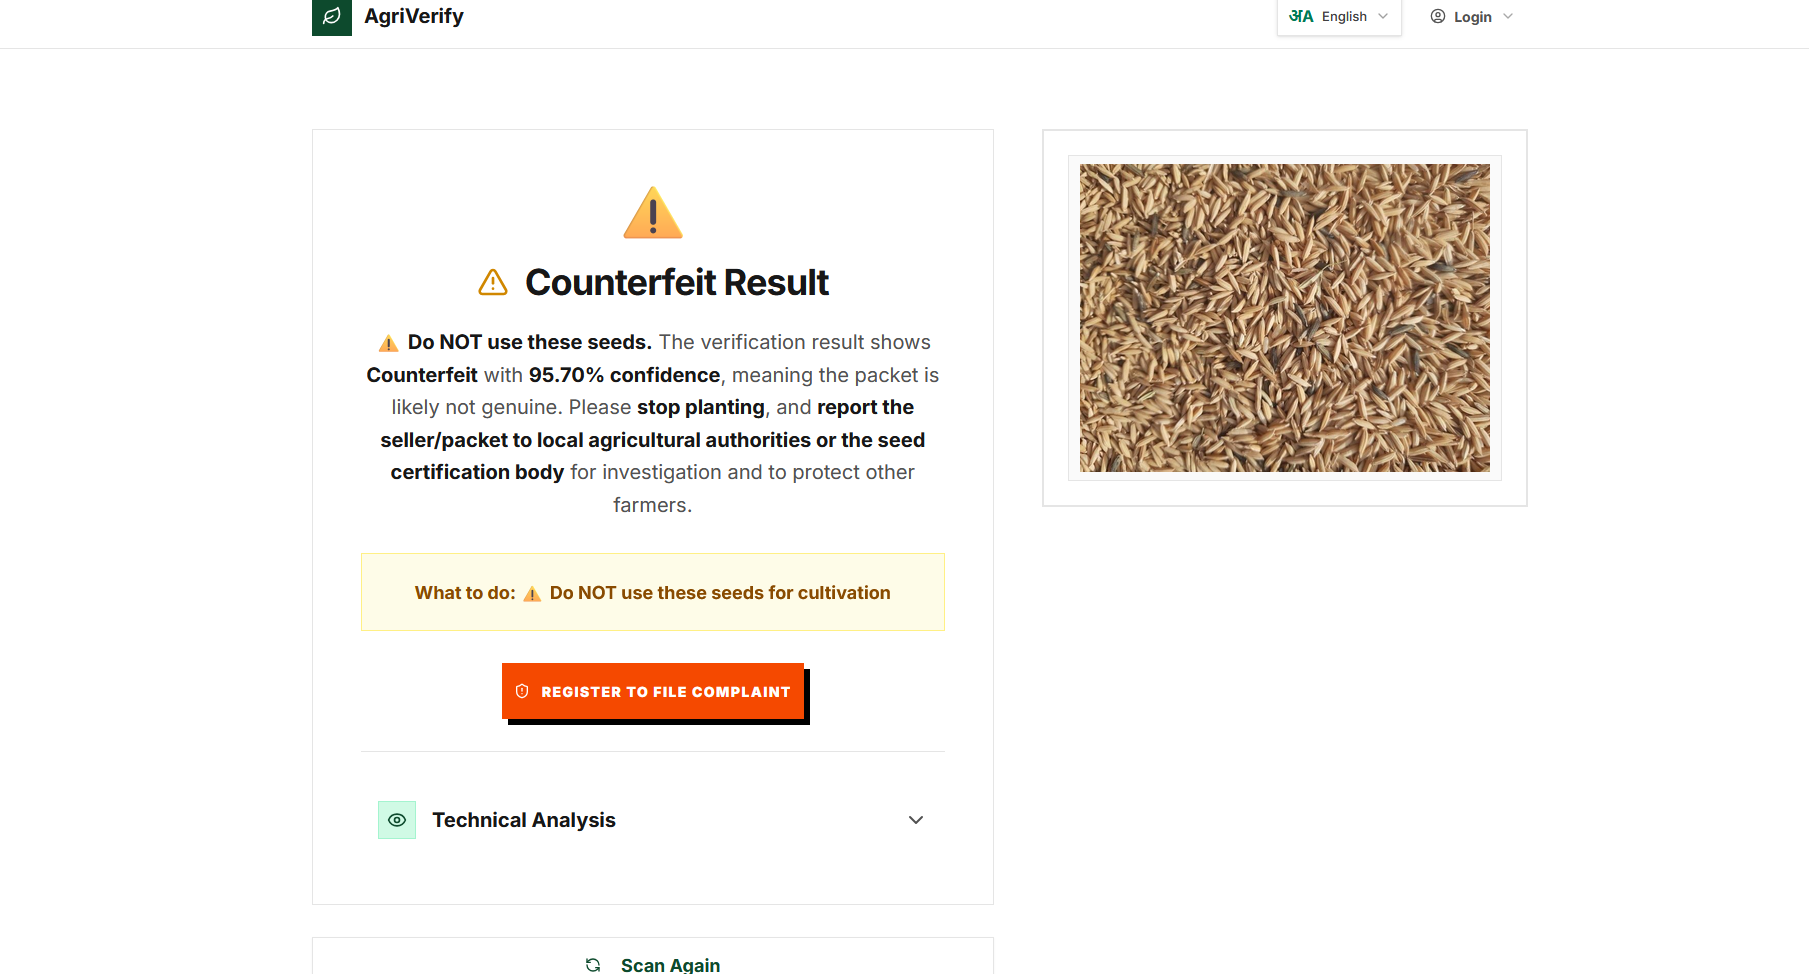
\includegraphics[width=\textwidth]{images/counterfeit.png}
  \caption{Verification alert for counterfeit or low-quality seed batch.}
  \label{fig:ui-counterfeit}
\end{figure}

\subsection{Grievance Redressal and Officer Investigation Interfaces}

In instances of quality failure or suspected counterfeit distribution, farmers can lodge formal complaints detailing the batch source and severity (Figure~\ref{fig:ui-complaints-form}). The status and resolution progress of these submissions can be monitored via the complaint queue interface (Figure~\ref{fig:ui-complaints-queue}).

\begin{figure}[htbp]
  \centering
  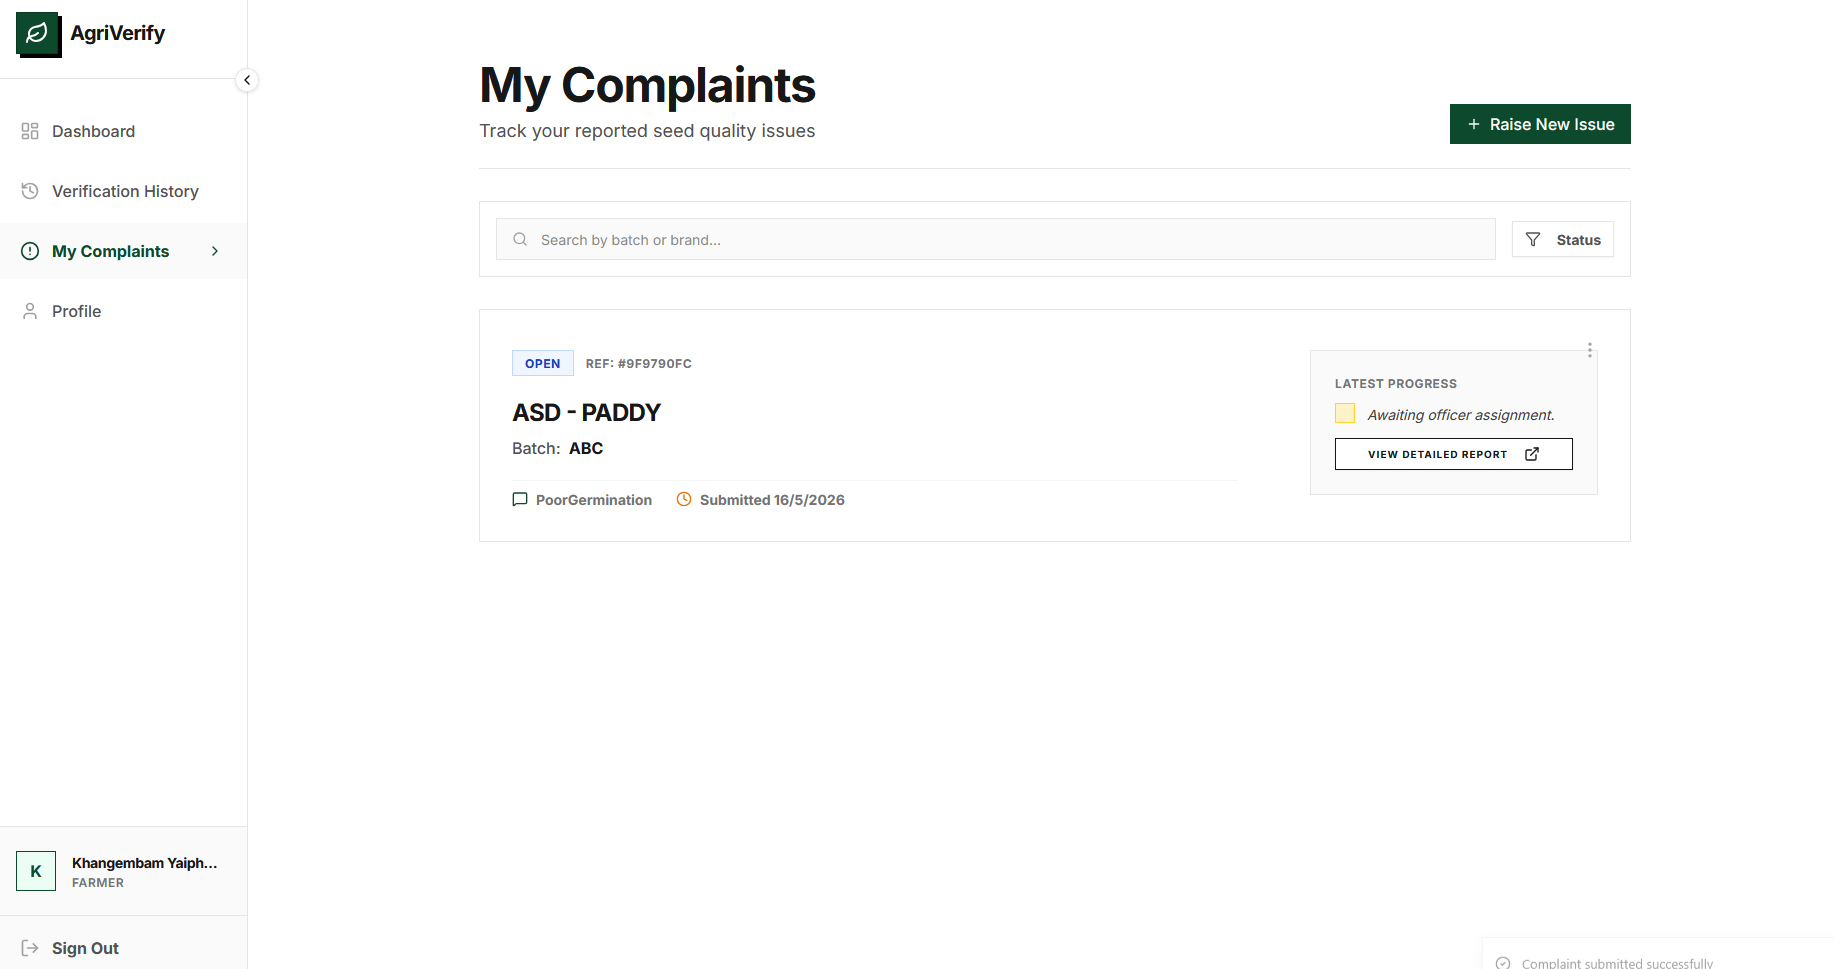
\includegraphics[width=\textwidth]{images/complains.png}
  \caption{Grievance registration interface for lodging seed quality complaints.}
  \label{fig:ui-complaints-form}
\end{figure}

\begin{figure}[htbp]
  \centering
  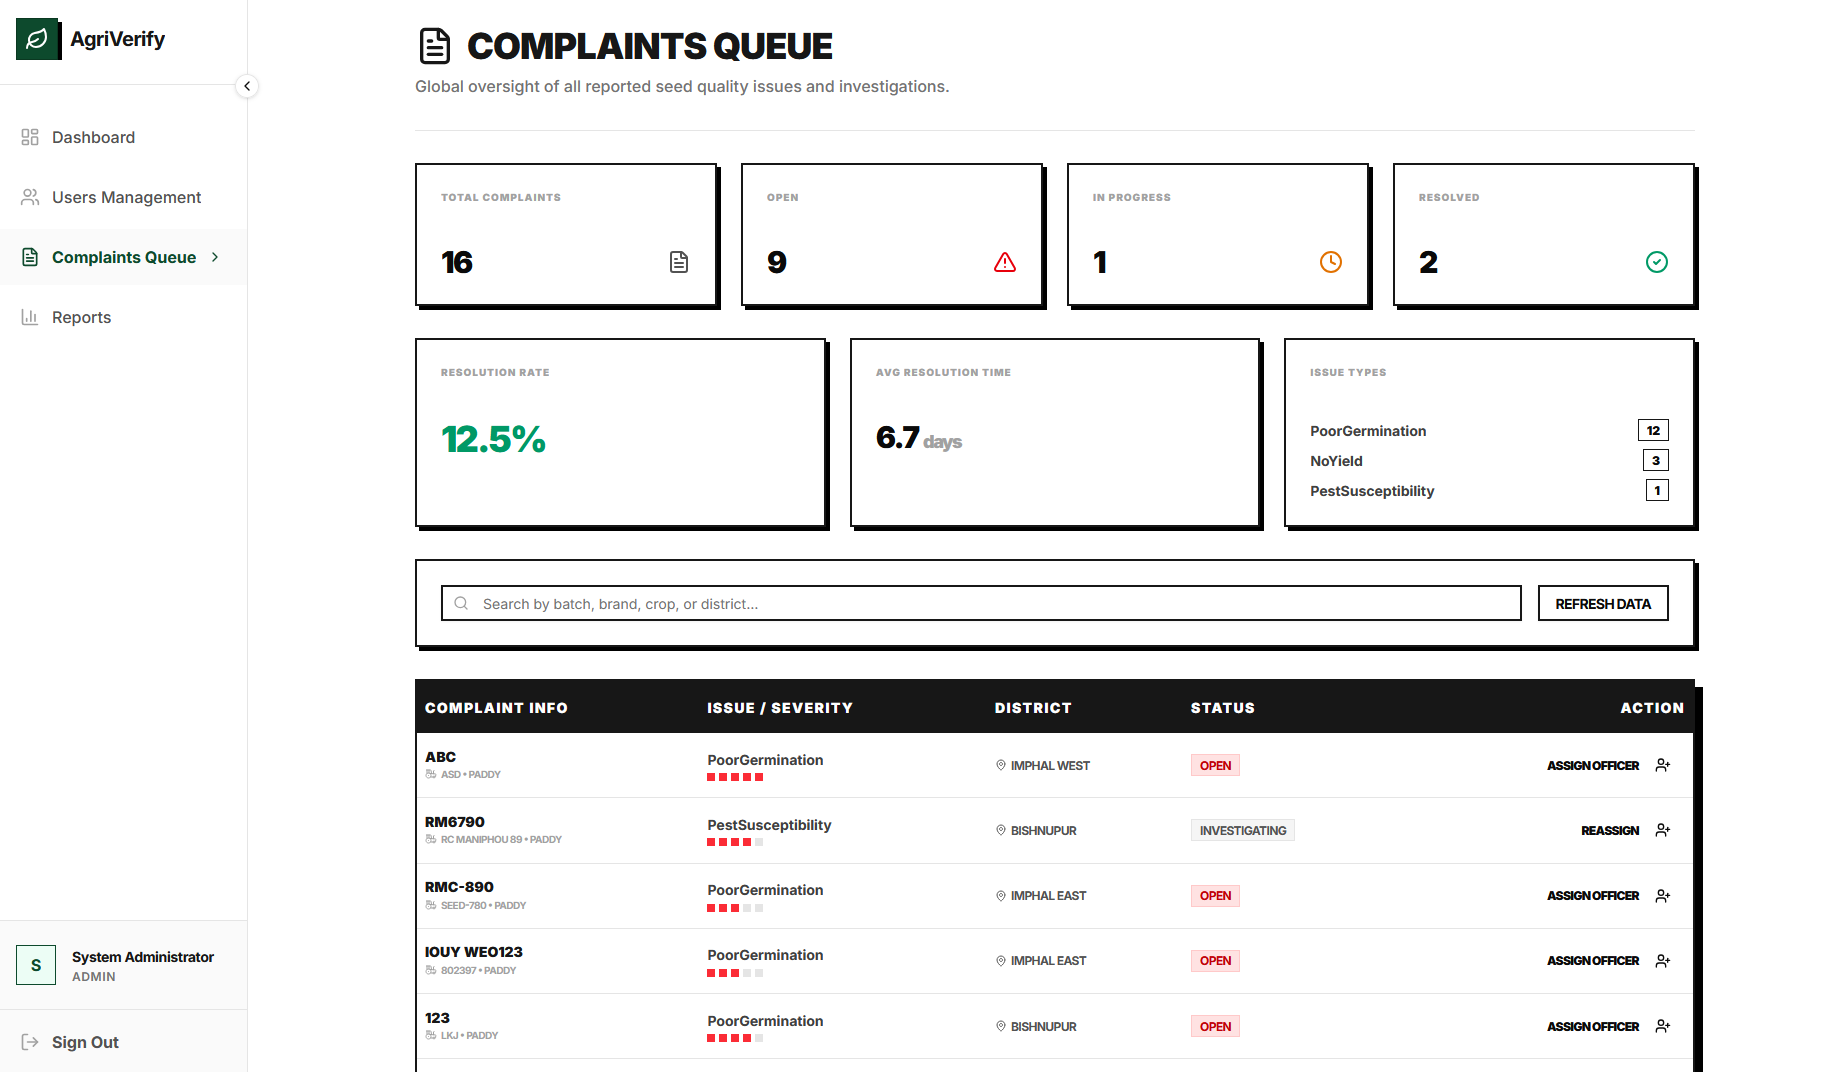
\includegraphics[width=\textwidth]{images/complains-queue.png}
  \caption{Farmer tracking interface for monitoring grievance status.}
  \label{fig:ui-complaints-queue}
\end{figure}

Agricultural officers access a dedicated monitoring dashboard summarizing regional complaints and workload distribution metrics (Figure~\ref{fig:ui-officer-dashboard}). Officers can query, filter, and prioritize the investigation queue based on severity, date, and location (Figure~\ref{fig:ui-investigation-queue}). Selecting a specific complaint displays the detailed investigation pane, allowing officers to examine user-submitted image evidence and update the resolution status (Figure~\ref{fig:ui-complaint-officer}).

\begin{figure}[htbp]
  \centering
  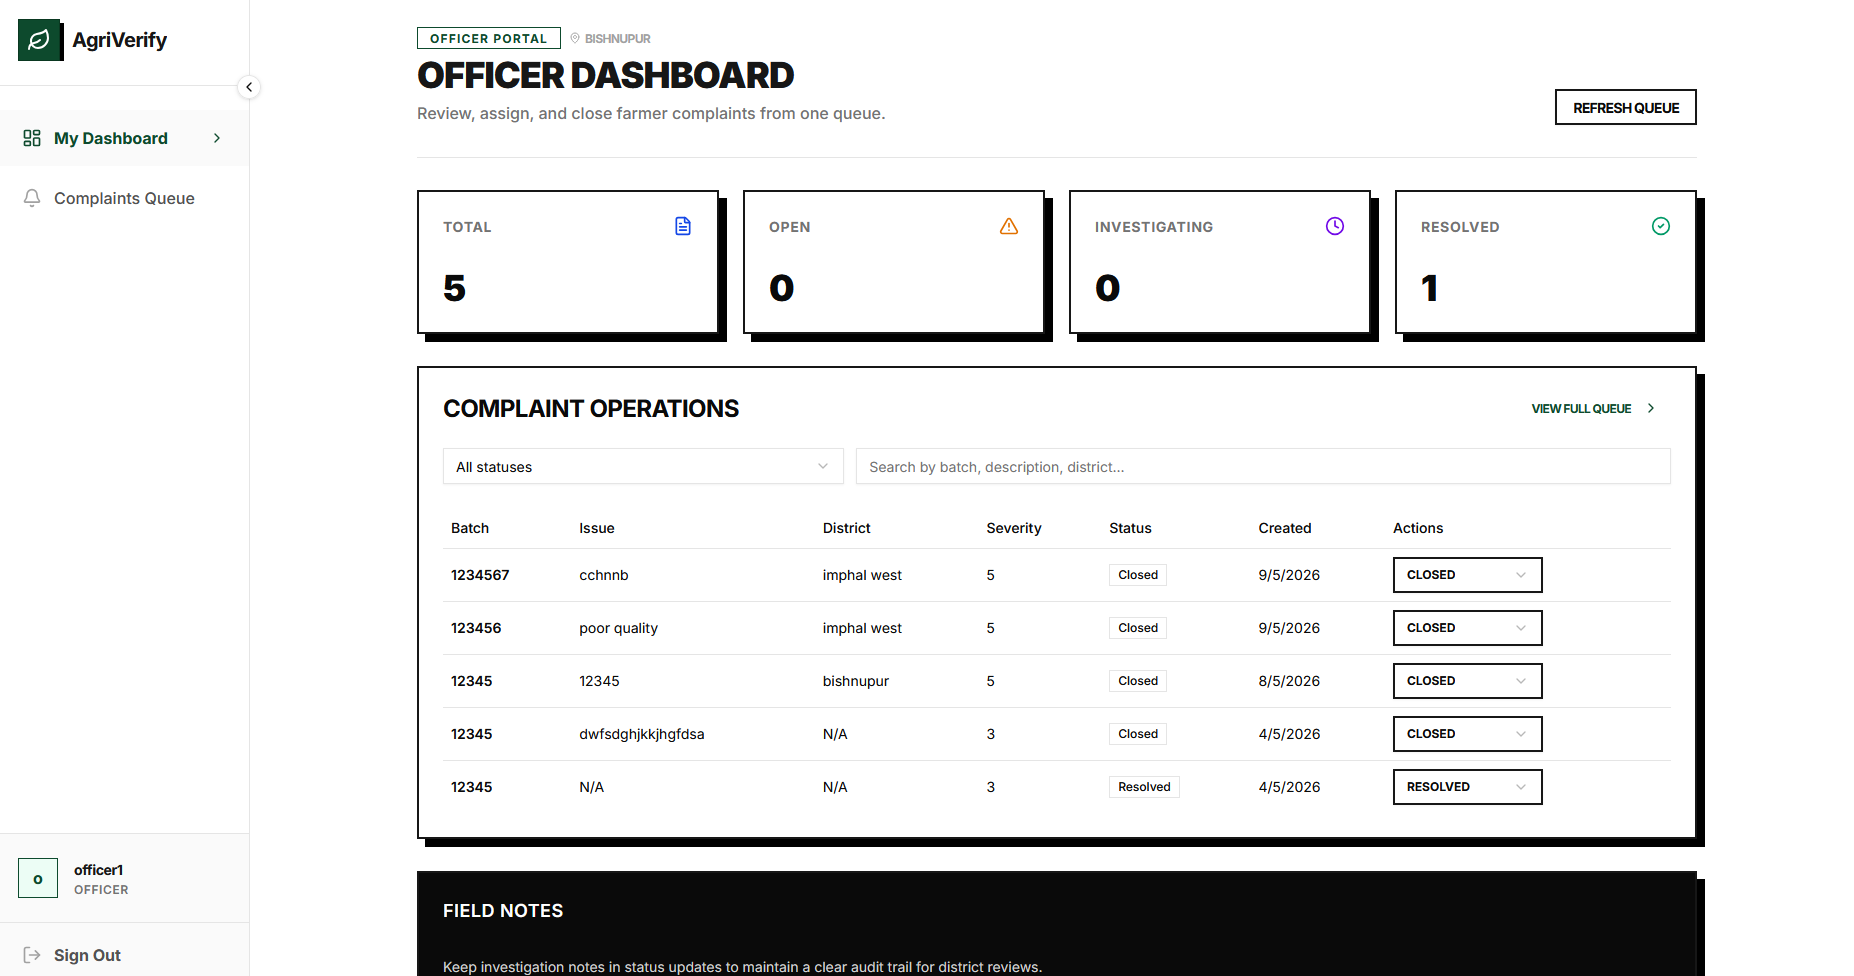
\includegraphics[width=\textwidth]{images/officer-dashboard.png}
  \caption{Agricultural officer dashboard presenting regional complaint metrics.}
  \label{fig:ui-officer-dashboard}
\end{figure}

\begin{figure}[htbp]
  \centering
  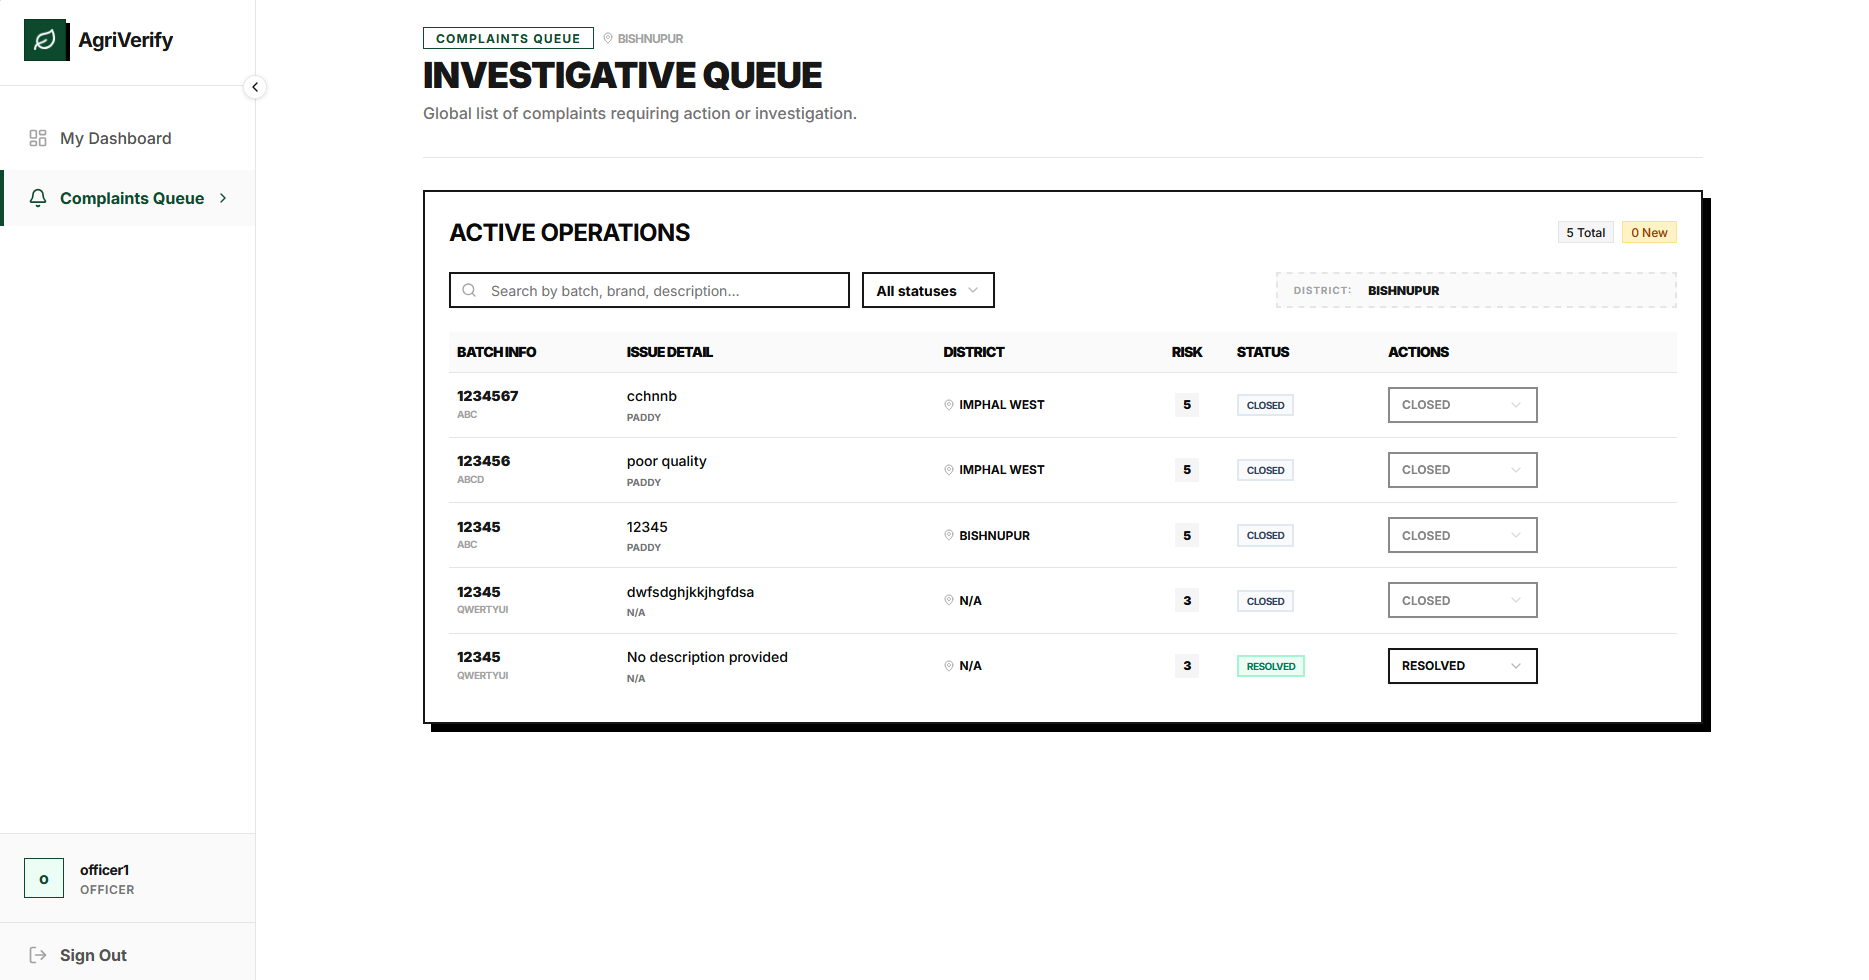
\includegraphics[width=\textwidth]{images/investigation-queue.png}
  \caption{Filtered and prioritized grievance investigation queue for officers.}
  \label{fig:ui-investigation-queue}
\end{figure}

\begin{figure}[htbp]
  \centering
  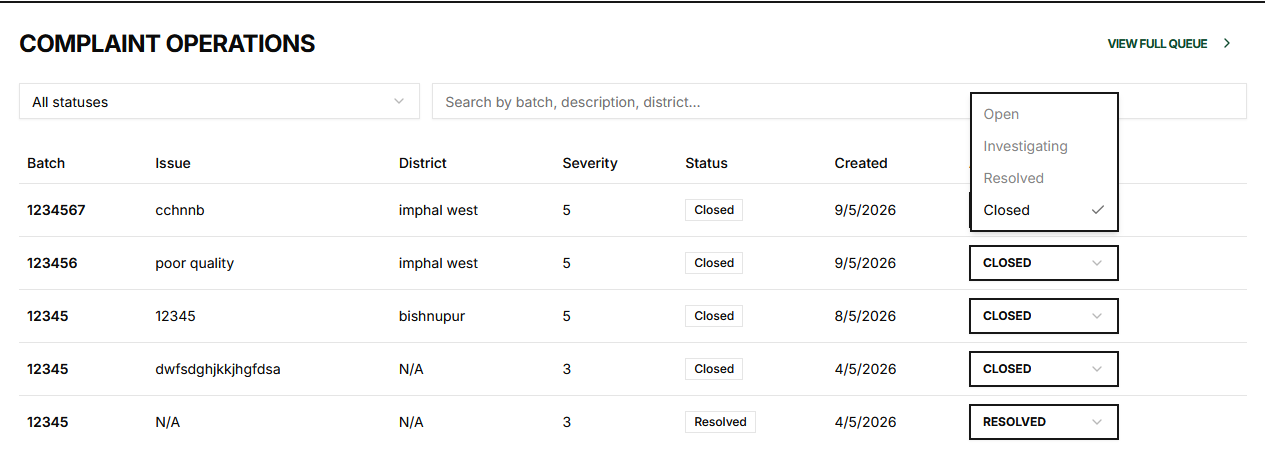
\includegraphics[width=\textwidth]{images/complains-officer.png}
  \caption{Officer grievance detail pane featuring user evidence and resolution controls.}
  \label{fig:ui-complaint-officer}
\end{figure}

\subsection{Platform Administration, User Governance, and Telemetry}

Platform administrators monitor system telemetry, API response times, active sessions, and database load via the real-time administrator dashboard (Figure~\ref{fig:ui-admin-dashboard}). Administrative user governance, including account creation and role modification, is managed through the user governance portal (Figure~\ref{fig:ui-user-mgmt}).

\begin{figure}[htbp]
  \centering
  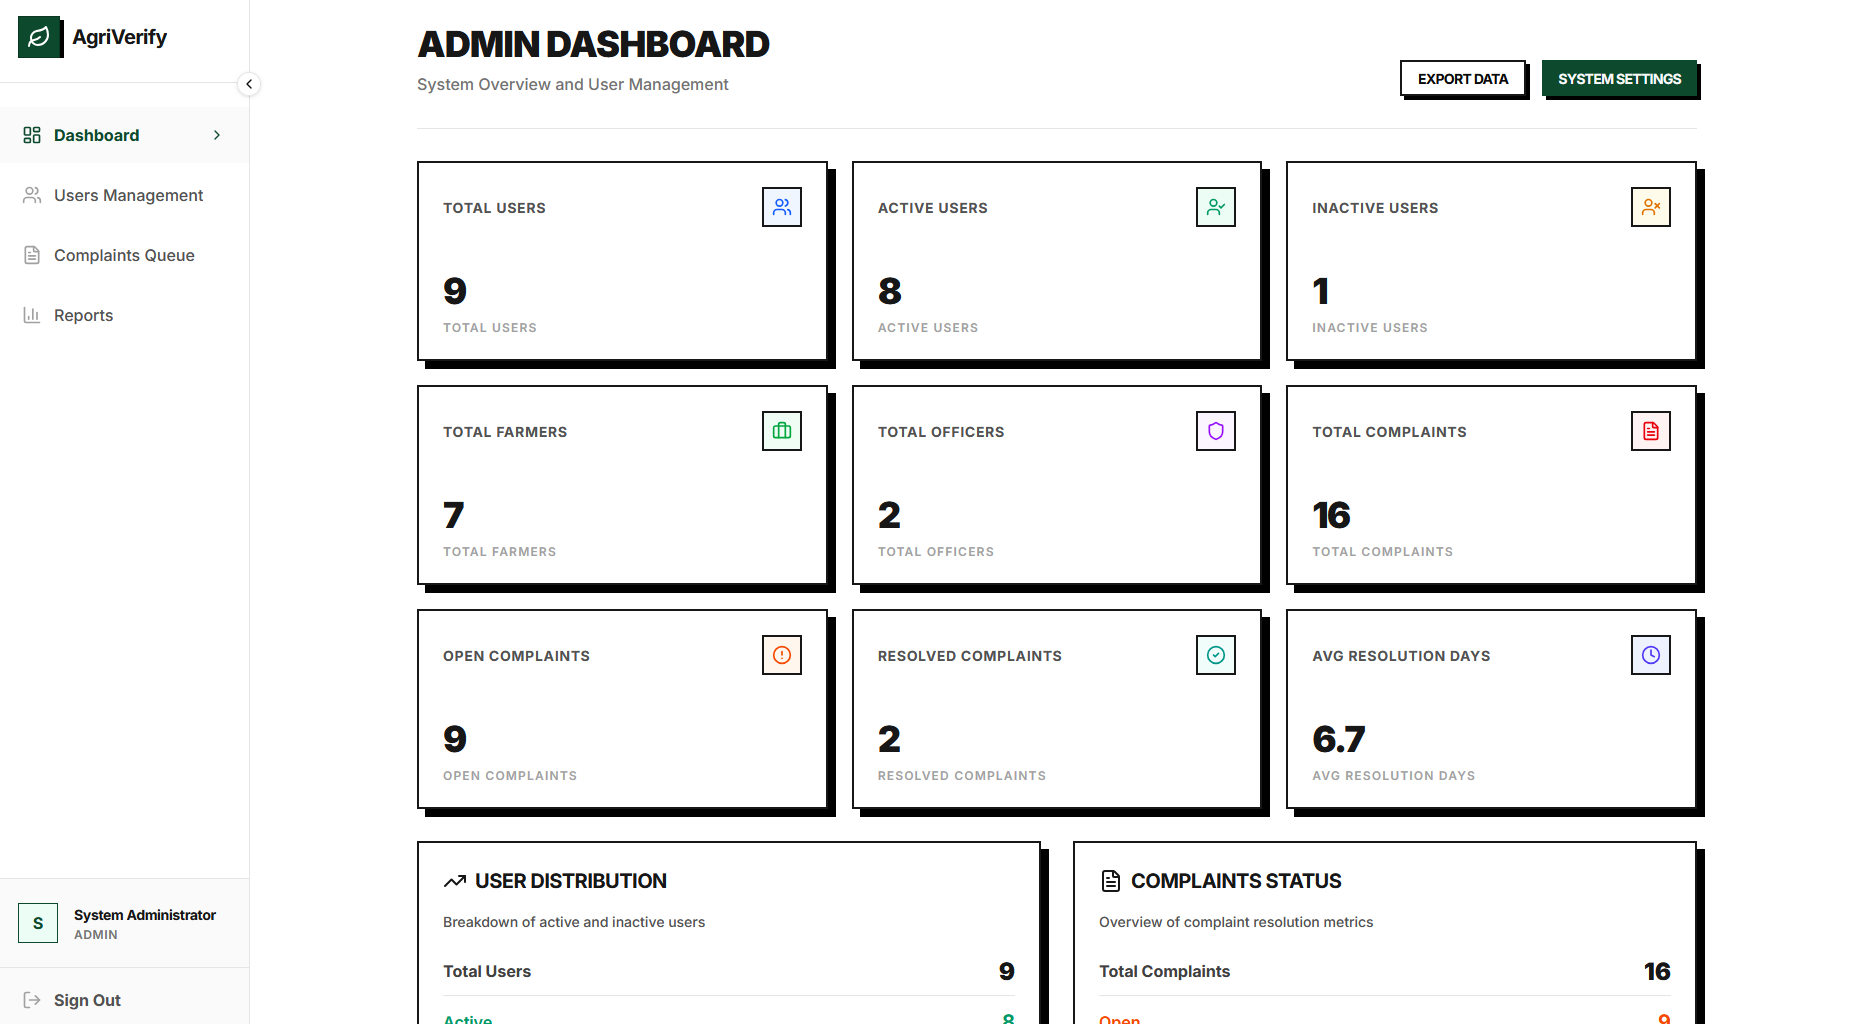
\includegraphics[width=\textwidth]{images/admin-dashboard.png}
  \caption{Administrator real-time system performance telemetry dashboard.}
  \label{fig:ui-admin-dashboard}
\end{figure}

\begin{figure}[htbp]
  \centering
  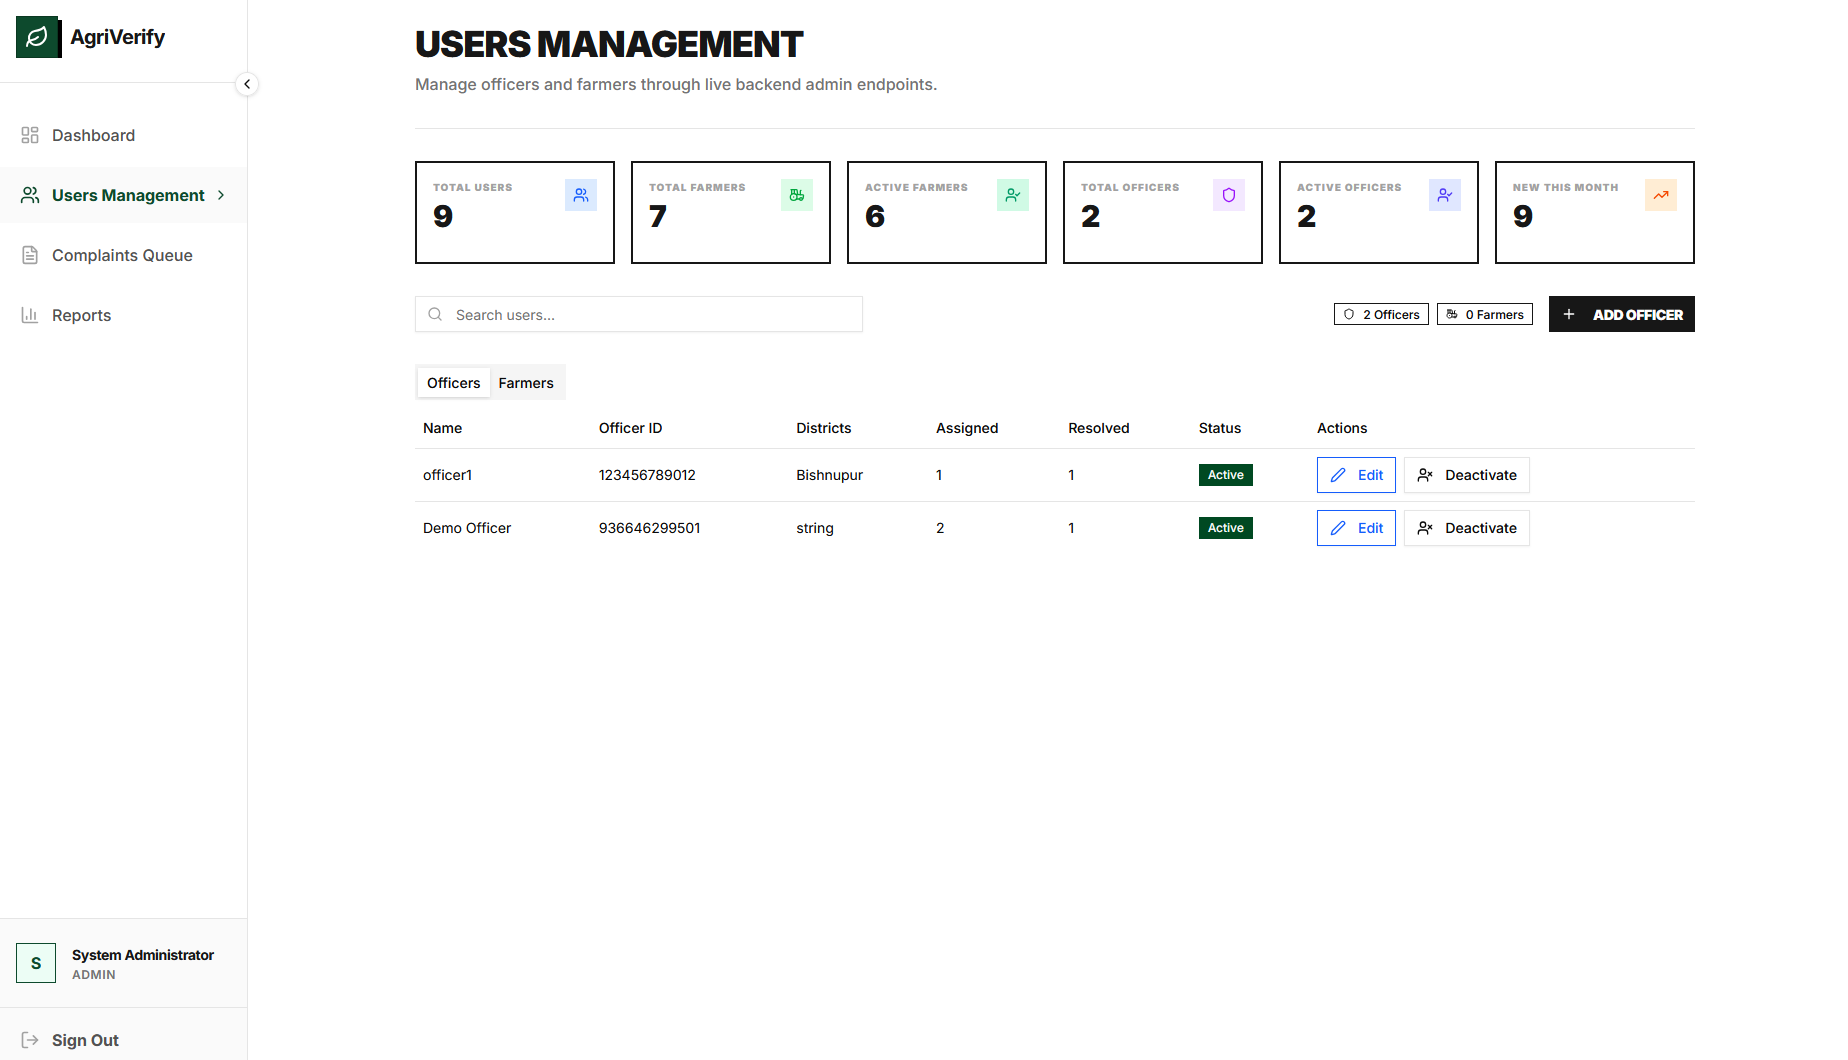
\includegraphics[width=\textwidth]{images/user-management.png}
  \caption{User administration and access control interface.}
  \label{fig:ui-user-mgmt}
\end{figure}

System analytics are visualized through reporting dashboards that highlight verification trends and fake seed detection rates over time (Figure~\ref{fig:ui-reports-1}). Geographical visualization dashboards map the distribution of counterfeit seed incidents across different administrative districts, aiding policymakers in identifying counterfeit hotspots (Figure~\ref{fig:ui-reports-2}).

\begin{figure}[htbp]
  \centering
  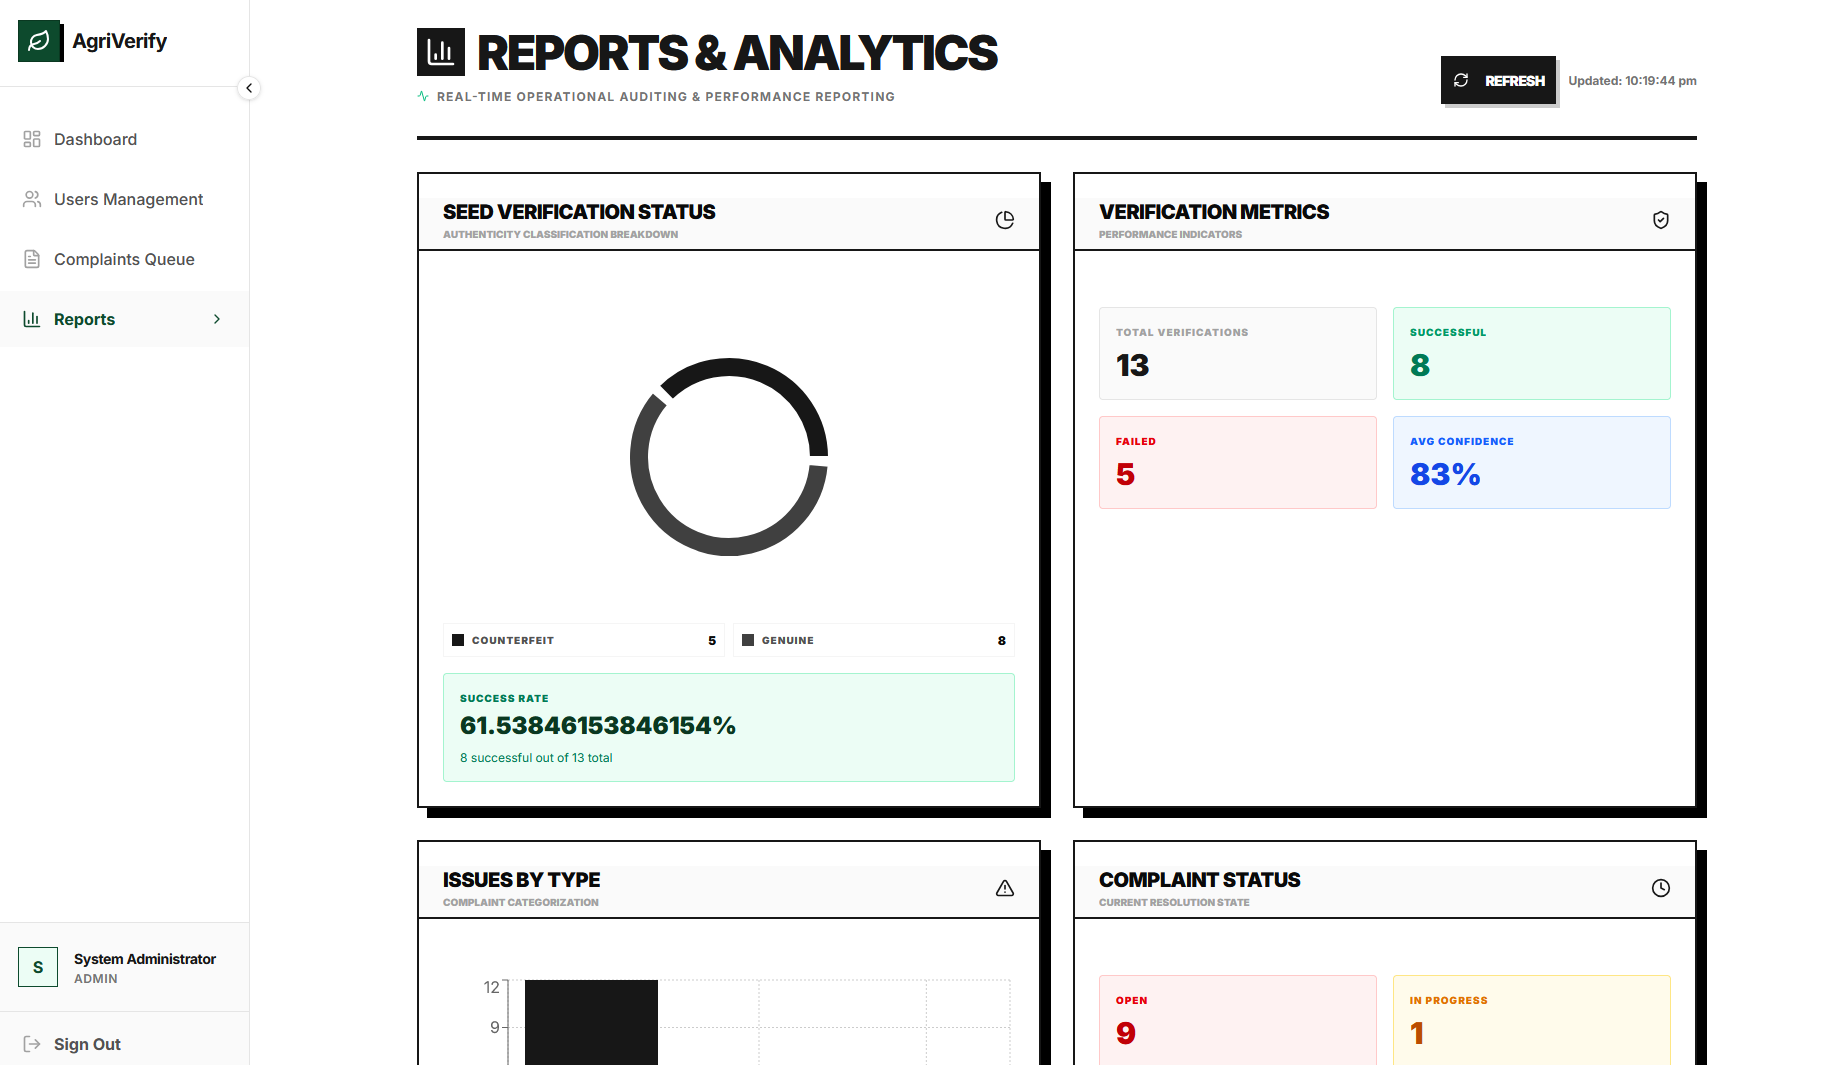
\includegraphics[width=\textwidth]{images/reports-and-analytics.png}
  \caption{Analytical reporting dashboard showing quality trends and system statistics.}
  \label{fig:ui-reports-1}
\end{figure}

\begin{figure}[htbp]
  \centering
  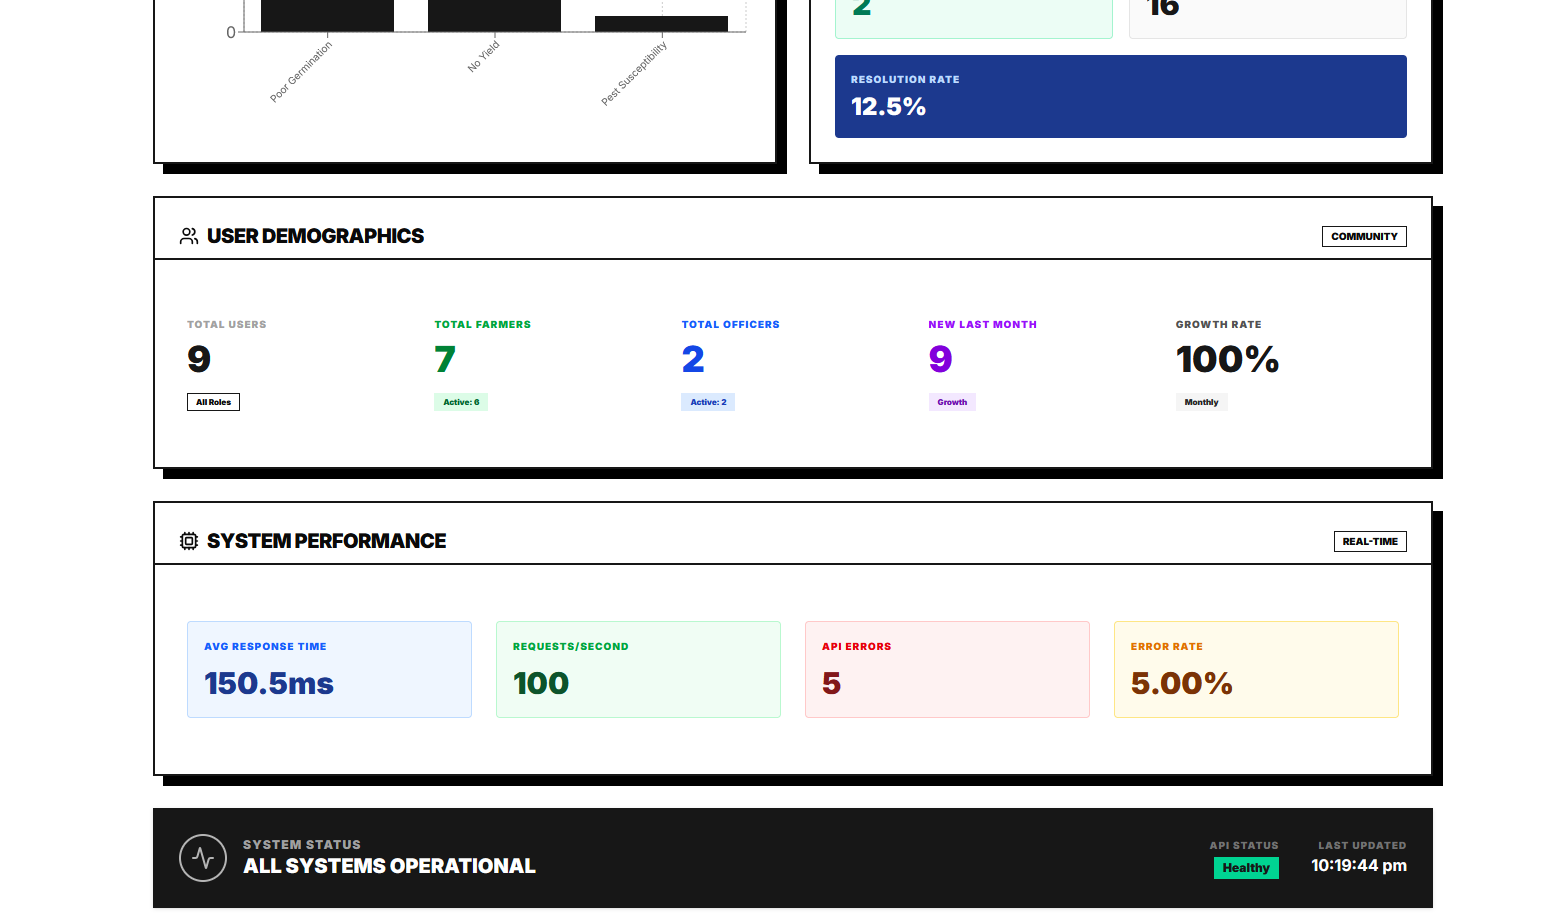
\includegraphics[width=\textwidth]{images/reports-and-analytics-2nd.png}
  \caption{District-wise geospatial hot-spot mapping of counterfeit occurrences.}
  \label{fig:ui-reports-2}
\end{figure}

% ──────────────────────────────────────────────────────────────
\section{Challenges Encountered and Mitigation Strategies}
\label{sec:challenges}
% ──────────────────────────────────────────────────────────────

The development and deployment of AgriVerify encountered several technical challenges, which were addressed using specific mitigation strategies:

\begin{itemize}
    \item \textbf{Data Scarcity:} The training dataset comprised only 1,563 images, introducing a high risk of model overfitting. This constraint was mitigated by utilizing transfer learning with pre-trained ImageNet weights, applying data augmentation to simulate sample diversity, and employing weight decay to regularize model complexity~\cite{krizhevsky2012imagenet, loshchilov2019adamw}.
    
    \item \textbf{Fine-Grained Feature Similarity:} Discriminating between mechanically damaged seeds and high-quality counterfeit packaging required high classification sensitivity. The system mitigated this by combining visual texture analysis with Optical Character Recognition (OCR) to extract text features from the packaging labels, providing multi-modal confirmation~\cite{mohanty2016}.
    
    \item \textbf{Environmental Illumination Variations:} Field photographs taken by farmers under uncontrolled ambient lighting conditions could degrade classification accuracy. To resolve this, automatic preprocessing algorithms adjust image contrast and brightness before inference, and training images were augmented with random color jittering to enhance model robustness.
    
    \item \textbf{Resource Constraints and Model Scale:} Deploying a standard ResNet50 model (approximately 100 MB) on edge servers introduces latency and memory bottlenecks. This was mitigated by implementing half-precision floating-point quantization (FP16) and model optimization, reducing memory footprints without compromising classification accuracy~\cite{pytorch2019}.
\end{itemize}

% ──────────────────────────────────────────────────────────────
\section{Summary and System Limitations}
\label{sec:limitations}
% ──────────────────────────────────────────────────────────────

This chapter presented a multi-dimensional evaluation of the AgriVerify platform, spanning model classification performance, system latency under concurrent loads, and functional validation. The ResNet50 classifier achieved an accuracy of 99.57\% and an F1 Score of 99.57\%, demonstrating performance in distinguishing certified seeds from damaged or counterfeit counterparts. Functional validation verified that the platform's core workflows operate correctly and securely.

Despite these positive results, several system limitations remain to be addressed in future work:

\begin{itemize}
    \item \textbf{Single-Crop Dependency:} The classifier is currently optimized exclusively for paddy seeds. Extending support to other major crops, such as wheat, maize, or soybeans, would require compiling specialized image datasets and retraining the network~\cite{xu2021}.
    
    \item \textbf{Network Connectivity Requirements:} The system relies on cloud-based API serving, restricting use in remote agricultural areas with poor internet connectivity. Quantizing models for offline, local execution on mobile devices represents a critical future development path.
    
    \item \textbf{Lack of Diagnostic Specificity:} While the system detects seed impurity, it does not identify specific seed-borne diseases or pathogens. Integrating phytopathological diagnostic capabilities would enhance agricultural value~\cite{mohanty2016}.
\end{itemize}

Addressing these limitations---through edge optimization, multi-crop expansion, and explainable AI (XAI) features to visualize classification attention maps---constitutes the primary roadmap for future research.